% Options for packages loaded elsewhere
\PassOptionsToPackage{unicode}{hyperref}
\PassOptionsToPackage{hyphens}{url}
%
\documentclass[
]{article}
\usepackage{amsmath,amssymb}
\usepackage{lmodern}
\usepackage{iftex}
\ifPDFTeX
  \usepackage[T1]{fontenc}
  \usepackage[utf8]{inputenc}
  \usepackage{textcomp} % provide euro and other symbols
\else % if luatex or xetex
  \usepackage{unicode-math}
  \defaultfontfeatures{Scale=MatchLowercase}
  \defaultfontfeatures[\rmfamily]{Ligatures=TeX,Scale=1}
\fi
% Use upquote if available, for straight quotes in verbatim environments
\IfFileExists{upquote.sty}{\usepackage{upquote}}{}
\IfFileExists{microtype.sty}{% use microtype if available
  \usepackage[]{microtype}
  \UseMicrotypeSet[protrusion]{basicmath} % disable protrusion for tt fonts
}{}
\makeatletter
\@ifundefined{KOMAClassName}{% if non-KOMA class
  \IfFileExists{parskip.sty}{%
    \usepackage{parskip}
  }{% else
    \setlength{\parindent}{0pt}
    \setlength{\parskip}{6pt plus 2pt minus 1pt}}
}{% if KOMA class
  \KOMAoptions{parskip=half}}
\makeatother
\usepackage{xcolor}
\usepackage[margin=1in]{geometry}
\usepackage{color}
\usepackage{fancyvrb}
\newcommand{\VerbBar}{|}
\newcommand{\VERB}{\Verb[commandchars=\\\{\}]}
\DefineVerbatimEnvironment{Highlighting}{Verbatim}{commandchars=\\\{\}}
% Add ',fontsize=\small' for more characters per line
\usepackage{framed}
\definecolor{shadecolor}{RGB}{248,248,248}
\newenvironment{Shaded}{\begin{snugshade}}{\end{snugshade}}
\newcommand{\AlertTok}[1]{\textcolor[rgb]{0.94,0.16,0.16}{#1}}
\newcommand{\AnnotationTok}[1]{\textcolor[rgb]{0.56,0.35,0.01}{\textbf{\textit{#1}}}}
\newcommand{\AttributeTok}[1]{\textcolor[rgb]{0.77,0.63,0.00}{#1}}
\newcommand{\BaseNTok}[1]{\textcolor[rgb]{0.00,0.00,0.81}{#1}}
\newcommand{\BuiltInTok}[1]{#1}
\newcommand{\CharTok}[1]{\textcolor[rgb]{0.31,0.60,0.02}{#1}}
\newcommand{\CommentTok}[1]{\textcolor[rgb]{0.56,0.35,0.01}{\textit{#1}}}
\newcommand{\CommentVarTok}[1]{\textcolor[rgb]{0.56,0.35,0.01}{\textbf{\textit{#1}}}}
\newcommand{\ConstantTok}[1]{\textcolor[rgb]{0.00,0.00,0.00}{#1}}
\newcommand{\ControlFlowTok}[1]{\textcolor[rgb]{0.13,0.29,0.53}{\textbf{#1}}}
\newcommand{\DataTypeTok}[1]{\textcolor[rgb]{0.13,0.29,0.53}{#1}}
\newcommand{\DecValTok}[1]{\textcolor[rgb]{0.00,0.00,0.81}{#1}}
\newcommand{\DocumentationTok}[1]{\textcolor[rgb]{0.56,0.35,0.01}{\textbf{\textit{#1}}}}
\newcommand{\ErrorTok}[1]{\textcolor[rgb]{0.64,0.00,0.00}{\textbf{#1}}}
\newcommand{\ExtensionTok}[1]{#1}
\newcommand{\FloatTok}[1]{\textcolor[rgb]{0.00,0.00,0.81}{#1}}
\newcommand{\FunctionTok}[1]{\textcolor[rgb]{0.00,0.00,0.00}{#1}}
\newcommand{\ImportTok}[1]{#1}
\newcommand{\InformationTok}[1]{\textcolor[rgb]{0.56,0.35,0.01}{\textbf{\textit{#1}}}}
\newcommand{\KeywordTok}[1]{\textcolor[rgb]{0.13,0.29,0.53}{\textbf{#1}}}
\newcommand{\NormalTok}[1]{#1}
\newcommand{\OperatorTok}[1]{\textcolor[rgb]{0.81,0.36,0.00}{\textbf{#1}}}
\newcommand{\OtherTok}[1]{\textcolor[rgb]{0.56,0.35,0.01}{#1}}
\newcommand{\PreprocessorTok}[1]{\textcolor[rgb]{0.56,0.35,0.01}{\textit{#1}}}
\newcommand{\RegionMarkerTok}[1]{#1}
\newcommand{\SpecialCharTok}[1]{\textcolor[rgb]{0.00,0.00,0.00}{#1}}
\newcommand{\SpecialStringTok}[1]{\textcolor[rgb]{0.31,0.60,0.02}{#1}}
\newcommand{\StringTok}[1]{\textcolor[rgb]{0.31,0.60,0.02}{#1}}
\newcommand{\VariableTok}[1]{\textcolor[rgb]{0.00,0.00,0.00}{#1}}
\newcommand{\VerbatimStringTok}[1]{\textcolor[rgb]{0.31,0.60,0.02}{#1}}
\newcommand{\WarningTok}[1]{\textcolor[rgb]{0.56,0.35,0.01}{\textbf{\textit{#1}}}}
\usepackage{graphicx}
\makeatletter
\def\maxwidth{\ifdim\Gin@nat@width>\linewidth\linewidth\else\Gin@nat@width\fi}
\def\maxheight{\ifdim\Gin@nat@height>\textheight\textheight\else\Gin@nat@height\fi}
\makeatother
% Scale images if necessary, so that they will not overflow the page
% margins by default, and it is still possible to overwrite the defaults
% using explicit options in \includegraphics[width, height, ...]{}
\setkeys{Gin}{width=\maxwidth,height=\maxheight,keepaspectratio}
% Set default figure placement to htbp
\makeatletter
\def\fps@figure{htbp}
\makeatother
\setlength{\emergencystretch}{3em} % prevent overfull lines
\providecommand{\tightlist}{%
  \setlength{\itemsep}{0pt}\setlength{\parskip}{0pt}}
\setcounter{secnumdepth}{-\maxdimen} % remove section numbering
\ifLuaTeX
  \usepackage{selnolig}  % disable illegal ligatures
\fi
\IfFileExists{bookmark.sty}{\usepackage{bookmark}}{\usepackage{hyperref}}
\IfFileExists{xurl.sty}{\usepackage{xurl}}{} % add URL line breaks if available
\urlstyle{same} % disable monospaced font for URLs
\hypersetup{
  pdftitle={Algoritma Academy: Classification 1},
  pdfauthor={Samuel Chan},
  hidelinks,
  pdfcreator={LaTeX via pandoc}}

\title{Algoritma Academy: Classification 1}
\author{Samuel Chan}
\date{15 November, 2022}

\begin{document}
\maketitle

\hypertarget{background}{%
\section{Background}\label{background}}

\hypertarget{algoritma}{%
\subsection{Algoritma}\label{algoritma}}

The following coursebook is produced by the team at
\href{https://algorit.ma}{Algoritma} for its Data Science Academy
workshops. The coursebook is intended for a restricted audience only,
i.e.~the individuals and organizations having received this coursebook
directly from the training organization. It may not be reproduced,
distributed, translated or adapted in any form outside these individuals
and organizations without permission.

Algoritma is a data science education center with bootcamp programs
offered in:

\begin{itemize}
\tightlist
\item
  Bahasa Indonesia (Jakarta campus)\\
\item
  English (Singapore campus)
\end{itemize}

\hypertarget{lifelong-learning-benefits}{%
\subsubsection{Lifelong Learning
Benefits}\label{lifelong-learning-benefits}}

If you're an active student or an alumni member, you also qualify for
all our future workshops, 100\% free of charge as part of your
\textbf{lifelong learning benefits}. It is a new initiative to help you
gain mastery and advance your knowledge in the field of data
visualization, machine learning, computer vision, natural language
processing (NLP) and other sub-fields of data science. All workshops
conducted by us (from 1-day to 5-day series) are available to you
free-of-charge, and the benefits \textbf{never expire}.

\hypertarget{second-edition}{%
\subsubsection{Second Edition}\label{second-edition}}

This coursebook is initially written in 2017.

This is the second edition, written in late August 2020. Some of the
code has been refactored to work with the latest major version of R,
version 4.0. I would like to thank the incredible instructor team at
Algoritma for their thorough input and assistance in the authoring and
reviewing process.

\hypertarget{libraries-and-setup}{%
\subsection{Libraries and Setup}\label{libraries-and-setup}}

We'll set-up caching for this notebook given how computationally
expensive some of the code we will write can get.

\begin{Shaded}
\begin{Highlighting}[]
\NormalTok{knitr}\SpecialCharTok{::}\NormalTok{opts\_chunk}\SpecialCharTok{$}\FunctionTok{set}\NormalTok{(}\AttributeTok{cache=}\ConstantTok{TRUE}\NormalTok{)}
\FunctionTok{options}\NormalTok{(}\AttributeTok{scipen =} \DecValTok{9999}\NormalTok{)}
\FunctionTok{rm}\NormalTok{(}\AttributeTok{list=}\FunctionTok{ls}\NormalTok{())}
\end{Highlighting}
\end{Shaded}

You will need to use \texttt{install.packages()} to install any packages
that are not already downloaded onto your machine. You then load the
package into your workspace using the \texttt{library()} function:

\begin{Shaded}
\begin{Highlighting}[]
\FunctionTok{library}\NormalTok{(gtools)}
\FunctionTok{library}\NormalTok{(gmodels)}
\FunctionTok{library}\NormalTok{(ggplot2)}
\FunctionTok{library}\NormalTok{(class)}
\end{Highlighting}
\end{Shaded}

\hypertarget{training-objectives}{%
\subsection{Training Objectives}\label{training-objectives}}

In this workshop, we'll extend our understanding of regression
algorithms and see what we've learned in the previous workshop can be
extended to solve a different kind of problems: classification problems.
More specifically, we'll learn to solve binary and multi-class
classification models using machine learning algorithms that are easily
understood and in the case of logistic regression, readily
interpretable.

You will learn to develop classification algorithms from scratch, and
investigate the mathematical foundations underpinning logistic
regressions and nearest neighbors algorithms. My objective is to deliver
a 9-hour session that is packed with the depth to help you develop,
apply, score and evaluate two of the most highly versatile algorithms
widely used today.

\begin{itemize}
\item
  \textbf{Logistic Regression}
\item
  Understanding Odds\\
\item
  Log of Odds\\
\item
  Sigmoid Curve\\
\item
  \texttt{glm} Function\\
\item
  Logistic Regression in Practice
\item
  \textbf{Nearest Neighbors Prediction}
\end{itemize}

\hypertarget{logistic-regression}{%
\section{Logistic Regression}\label{logistic-regression}}

\hypertarget{theory}{%
\subsection{Theory}\label{theory}}

Logistic regression is a classification algorithm used to fit a
regression curve, \(y = f(x)\), where \(y\) is a categorical variable.
When \(y\) is binary (1 for spam, 0 for not-spam) we also call the model
\textbf{binomial logistic regression} where in cases of \(y\) assuming
more than 2 values you'll sometimes hear the model being referred to as
a class of \textbf{multinomial logistic regression}. We can think of
logistic regression as a special case of linear regression (which you've
mastered in the previous workshop), except we're using \textbf{log of
odds} as our target variable.

\hypertarget{relation-to-probability}{%
\subsection{Relation to Probability}\label{relation-to-probability}}

So it's perhaps important to understand what odds mean. Most of us are
familiar with \textbf{probabilities}. We understood that the
\textbf{probability} of an event is the proportion of times it will
occur divided by the total number of trials. If an event occurs 1 out of
5 times, then the probability (\texttt{p}) would be 1 out of 5, or 0.2.

Odds are defined as the probability that an event will occur
(\texttt{p}) divided by the probability than the event will not occur
(we'll call it \texttt{q}, which is the same as \texttt{1-p}). If p is
0.2, we will see that q is 0.8. Expressed in a formula, odds can then be
defined as:\\
\(\frac{p}{(1-p)}\)

Let's use a fun and real-life example. Supposed we were playing black
jack (assuming the casino uses two decks on black jack) and the first
card dealt is an Ace, the probability of the next card dealt to the
dealer is a Ten is 31.07\% (32 possible Tens out of 103 possibility). If
we have to express it in odds and define p as 0.31, then our odds of the
dealer being dealt a Blackjack (Ace + a Ten) is 0.31/(1-0.31), which
brings it to 0.45 to 1.

Note that if we have defined \texttt{p} as the probability of the Dealer
\textbf{not having a Blackjack}, our odds would instead be 0.69/0.31,
which brings us to 2.23 to 1. We can interpret this as ``for every 2.23
times the dealer didn't get a blackjack, she would get 1 blackjack''.
Odds, as we so far understand it, refers to the ratio of favorable event
(dealer doesn't get a blackjack) to the unfavorable event.

\textbf{Quiz 1: Odds of flying on time vs suffering a departure delay}

Now to a less-fun but no less important example: airport delays. If I
tell you that the probability of a minor departure delay occurring at a
particularly busy airport (Soekarno-Hatta) on a festive holiday season
is 0.2, what are the chances (expressed in odds) of you departing on
time versus that of a departure delay. Recall the formula:

\(Odds = \frac{No-delay}{Delay}\)

I hope you arrived at the right answer of 4 to 1, and intuitively
interpret the situation as ``we are 4 times more likely to depart on
time than to be delayed''.

Odds are rather commonly used in some industry and in sports. In
football and in horse racing, you'll often see betting odds expressed as
fractions (e.g.~3/1 for a Germany win). In some academic writing or
journalistic reporting, you may also see odds being expressed such as
this: ``the relative risk of a credit event with Financial Product A
over Product B is 1.125''. If you think about it, this is the same
concept we've been talking about: odds.

If it wasn't immediately clear, consider assigning some numbers to the
above example:\\
- Financial Product A has a 0.45 empirical probability of incurring a
credit event\\
- Financial Product B has a 0.4 empirical probability of incurring a
credit event

The odds is hence 0.45/0.4, or 1.125:1.

\hypertarget{understanding-log-of-odds}{%
\subsubsection{Understanding log of
odds}\label{understanding-log-of-odds}}

When we have a probability \(p\), the log of odds (sometimes called the
``log-odds'') is simply the log of the odds ratio, which is:\\
\(log(p/(1-p))\)

Odds ratios as we observe above, are just an alternate way of expressing
probabilities. Let's say we have the probability of success as 0.8, then
the probability of failure is 1 - 0.8 = 0.2. The odds of success are
defined as the probability of success over the probability of failure,
in our case the odds would be .8/.2 = 4. We can also say that the odds
of success is hence 4 to 1. If the probability of success is .5, i.e
50-50, our odds of success is 1 to 1.

The transformation from probability to odds is a monotonic
transformation, so the odds increases as the probability increase
(however note that odds take a range of 0 to infinity):

\begin{Shaded}
\begin{Highlighting}[]
\FunctionTok{curve}\NormalTok{((x}\SpecialCharTok{/}\NormalTok{(}\DecValTok{1}\SpecialCharTok{{-}}\NormalTok{x)), }\AttributeTok{from =} \DecValTok{0}\NormalTok{, }\AttributeTok{to=}\DecValTok{1}\NormalTok{, }\AttributeTok{ylim=}\FunctionTok{c}\NormalTok{(}\DecValTok{0}\NormalTok{,}\DecValTok{10}\NormalTok{), }\AttributeTok{xlab =} \StringTok{"Probability"}\NormalTok{, }\AttributeTok{ylab=}\StringTok{"Odds"}\NormalTok{)}
\end{Highlighting}
\end{Shaded}

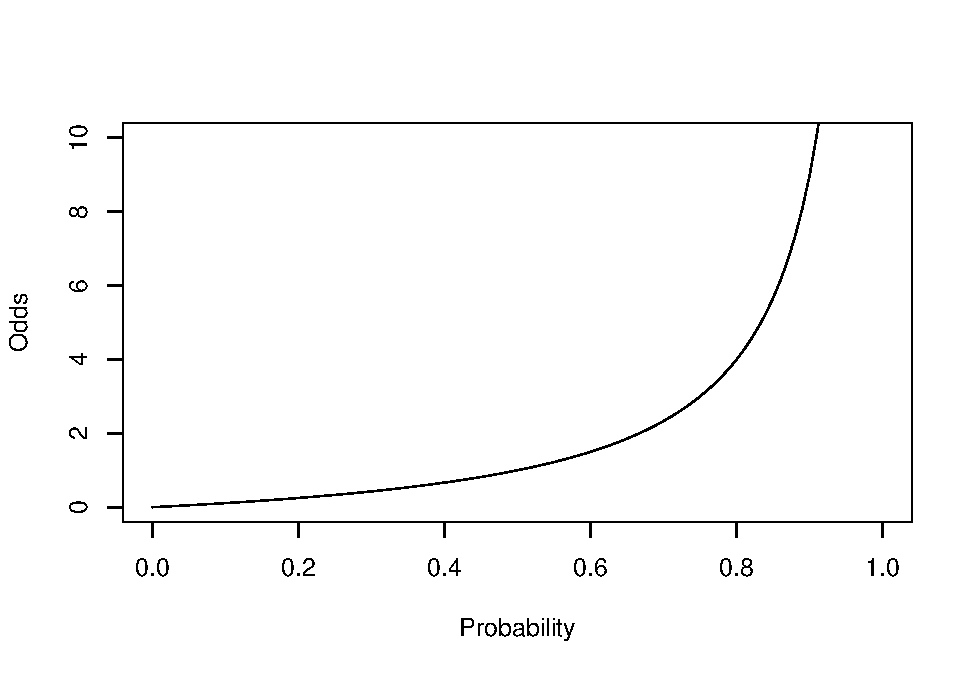
\includegraphics{classification1_files/figure-latex/unnamed-chunk-2-1.pdf}

Notice how we have an \textbf{odd of 1 when our p is 0.5}, and our odd
is 4, when p is 0.8, just as we learned from the earlier example (50:50
-\textgreater{} odds of 1, success rate of 0.8 -\textgreater{} odds of
4).

Now that we've understood the transformation from probability to odds,
let's understand the transformation from odds to logs of odds.

Log of odds are: \(logit(p) = log(\frac{p}{1-p})\)

Almost same code for the above curve, except this time we plot the curve
of \texttt{log(x/(1-x))} instead of \texttt{(x/(1-x))}.

\begin{Shaded}
\begin{Highlighting}[]
\CommentTok{\# Plot sigmoid curve}
\FunctionTok{curve}\NormalTok{(}\FunctionTok{log}\NormalTok{(x}\SpecialCharTok{/}\NormalTok{ (}\DecValTok{1}\SpecialCharTok{{-}}\NormalTok{x)), }\AttributeTok{from =} \DecValTok{0}\NormalTok{, }\AttributeTok{to=}\DecValTok{1}\NormalTok{, }\AttributeTok{xlab =} \StringTok{"Probability"}\NormalTok{, }\AttributeTok{ylab=}\StringTok{"Log of odds"}\NormalTok{)}
\end{Highlighting}
\end{Shaded}

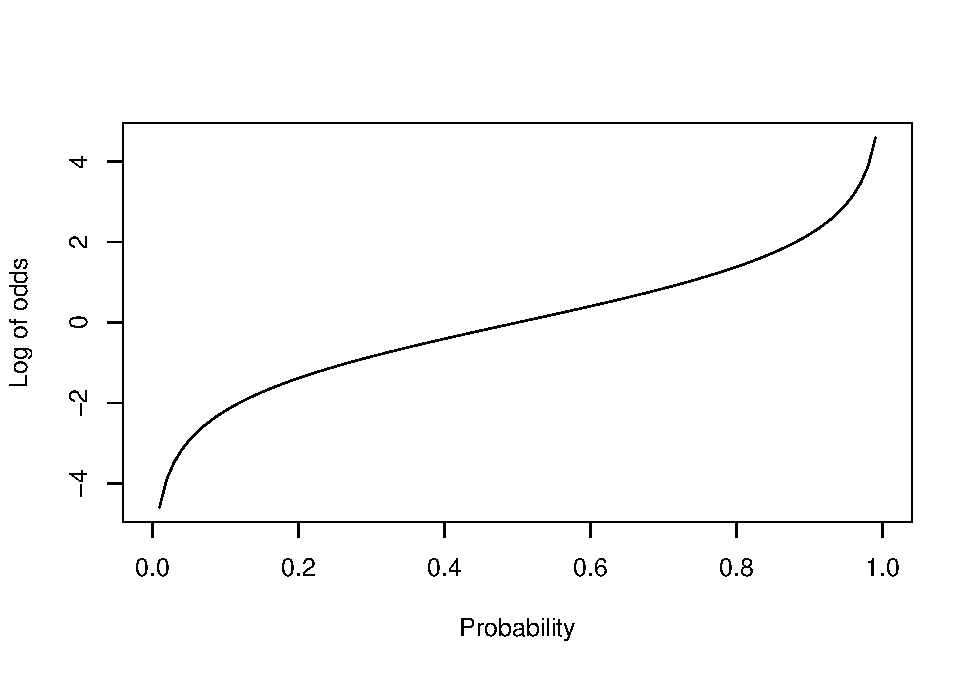
\includegraphics{classification1_files/figure-latex/unnamed-chunk-3-1.pdf}

Change \texttt{x} below from 0.5 to 1, and then to 0 to verify that the
log of odds can take any positive or negative value (which is to say,
its range is -Inf to Inf). A linear model can produce any value of log
of odds and they would be acceptable as a prediction as the range is
-Inf to Inf. That is not the case if a linear model has to produce a
prediction that is a valid value of ``probability'', because a
probability only takes a range of 0 to 1.

\begin{Shaded}
\begin{Highlighting}[]
\NormalTok{x }\OtherTok{\textless{}{-}} \FloatTok{0.5}
\FunctionTok{log}\NormalTok{(x}\SpecialCharTok{/}\NormalTok{ (}\DecValTok{1}\SpecialCharTok{{-}}\NormalTok{x))}
\end{Highlighting}
\end{Shaded}

\begin{verbatim}
## [1] 0
\end{verbatim}

Again, the transformation of odds to log of odds is a monotonic one. The
greater the odds, the greater the log of odds. However, recall that the
probability of .5 will yield us a log-odds of 0. This is because the
logit (log of odds) function takes values on {[}min, max{]} and
transforms them to span {[}-Inf, Inf{]}. 5 is our median number and
hence it's value on the log of odds scale is 0.

The above sigmoid curve can also be plotted using the \texttt{logit()}
function from the \texttt{gtools} package:

\begin{Shaded}
\begin{Highlighting}[]
\FunctionTok{library}\NormalTok{(gtools)}
\CommentTok{\# Plot sigmoid curve}
\CommentTok{\# logit(x) == log(x/(1{-}x))}
\FunctionTok{curve}\NormalTok{(}\FunctionTok{logit}\NormalTok{(x), }\AttributeTok{from =} \DecValTok{0}\NormalTok{, }\AttributeTok{to=}\DecValTok{1}\NormalTok{, }\AttributeTok{xlab =} \StringTok{"Probability"}\NormalTok{, }\AttributeTok{ylab=}\StringTok{"Log of odds"}\NormalTok{)}
\end{Highlighting}
\end{Shaded}

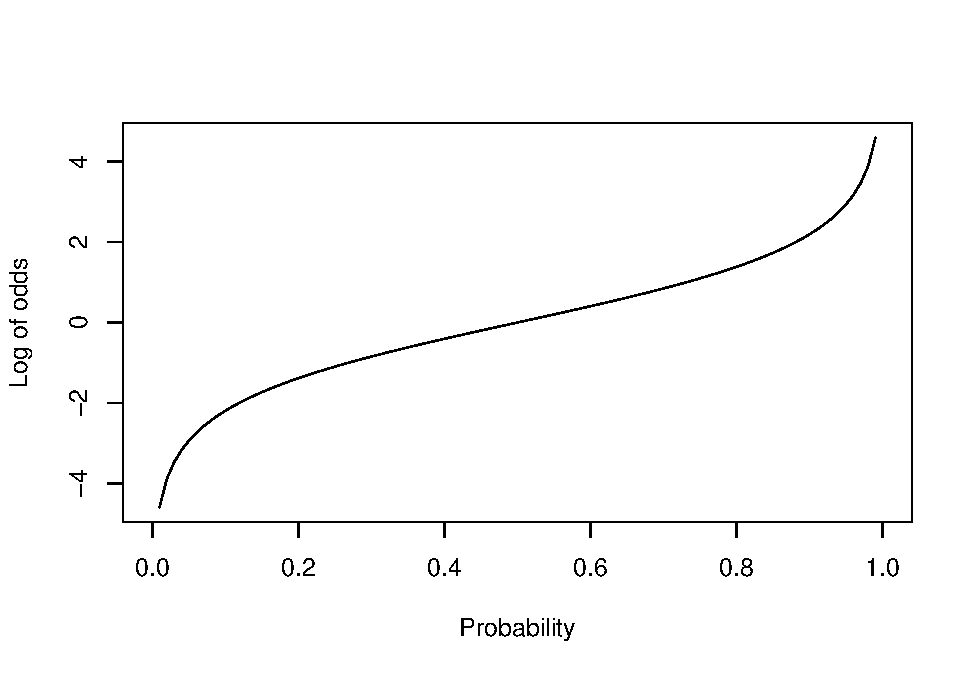
\includegraphics{classification1_files/figure-latex/unnamed-chunk-5-1.pdf}

\hypertarget{understanding-logit}{%
\subsubsection{\texorpdfstring{Understanding
\texttt{logit()}}{Understanding logit()}}\label{understanding-logit}}

The \texttt{logit} function, formally defined, is expressed as:
\(y = log(\frac{p}{1-p})\) where \(p = \frac{x - min}{max-min}\)

In the case of a p=0.5 on a scale of 0 to 1, our \emph{p} would then be
p = ( 0.5 - 0 ) / (1 - 0) = 0.5; In the case of a p=30 on a scale of 1
to 100, our \emph{p} would subsequently take on the value of
(30-1)/(100-1) = 0.292929293.

We can use the \texttt{logit()} function from the \texttt{gtools}
package, or just use \texttt{log()} with our odds and you'll get the
same result. What you obtained is the log of odds:

\begin{Shaded}
\begin{Highlighting}[]
\CommentTok{\# Proof}
\DocumentationTok{\#\# using logit(p, wo/ normalization)}
\NormalTok{proof1 }\OtherTok{\textless{}{-}} \FunctionTok{logit}\NormalTok{(}\DecValTok{30}\NormalTok{, }\AttributeTok{min=}\DecValTok{1}\NormalTok{, }\AttributeTok{max=}\DecValTok{100}\NormalTok{)}

\DocumentationTok{\#\# using logit(p, w/ min{-}max normalization)}
\NormalTok{proof2 }\OtherTok{\textless{}{-}} \FunctionTok{logit}\NormalTok{(}\FloatTok{0.292929293}\NormalTok{)}

\DocumentationTok{\#\# equivalent: log(p/(1{-}p))}
\NormalTok{proof3 }\OtherTok{\textless{}{-}} \FunctionTok{log}\NormalTok{(}\FloatTok{0.292929293}\SpecialCharTok{/}\NormalTok{(}\DecValTok{1}\FloatTok{{-}0.292929293}\NormalTok{))}

\NormalTok{proof1 }\OtherTok{\textless{}{-}} \FunctionTok{round}\NormalTok{(proof1, }\DecValTok{4}\NormalTok{)}
\NormalTok{proof2 }\OtherTok{\textless{}{-}} \FunctionTok{round}\NormalTok{(proof2, }\DecValTok{4}\NormalTok{)}
\NormalTok{proof3 }\OtherTok{\textless{}{-}} \FunctionTok{round}\NormalTok{(proof3, }\DecValTok{4}\NormalTok{)}

\FunctionTok{print}\NormalTok{(}\FunctionTok{paste}\NormalTok{(proof1, }\StringTok{" | "}\NormalTok{, proof2, }\StringTok{" | "}\NormalTok{, proof3))}
\end{Highlighting}
\end{Shaded}

\begin{verbatim}
## [1] "-0.8812  |  -0.8812  |  -0.8812"
\end{verbatim}

Notice, however, that the \texttt{logit} function puts our probability
on the x-axis instead of the y-axis and we can \emph{invert} both axes
by using the \texttt{inv.logit} function, also called the Sigmoidal
\textbf{logistic function}.

\begin{Shaded}
\begin{Highlighting}[]
\FunctionTok{library}\NormalTok{(gtools)}
\CommentTok{\# Plot sigmoid curve}
\FunctionTok{curve}\NormalTok{(}\FunctionTok{inv.logit}\NormalTok{(x), }\AttributeTok{from =} \SpecialCharTok{{-}}\DecValTok{10}\NormalTok{, }\AttributeTok{to=}\DecValTok{10}\NormalTok{)}
\end{Highlighting}
\end{Shaded}

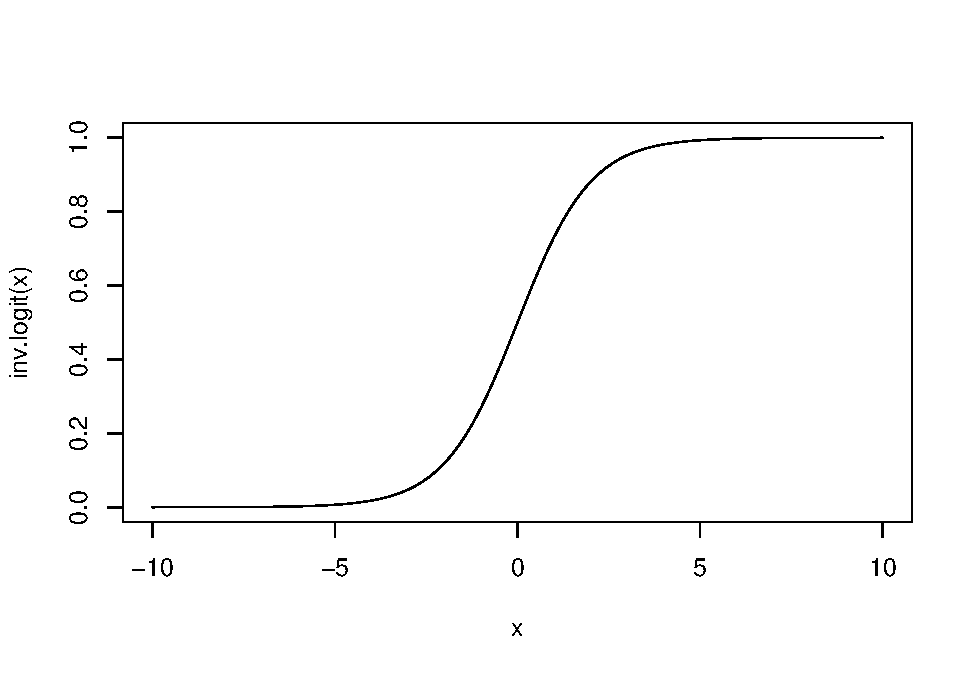
\includegraphics{classification1_files/figure-latex/unnamed-chunk-7-1.pdf}

You could be wondering by now why we're concerned with understanding
these underlying concepts? It turns out that the reason is surprisingly
straightforward if we approach it from our prior knowledge of linear
regression models.

Recall that with linear regression, we are used to representing our
hypothesis in the following form:

\(\hat{y} = \beta_0 + \beta_1x_1 + ... + \beta_mx_m\)\\
Where m is the number of predictors

But with that hypothesis, our value \(\hat{y}\) could take on any value
from \emph{-Inf} to \emph{Inf}. This is obviously not very helpful for
our classification task. Ideally, we want:

\(0 \leq \hat{y} \leq 1\)

This is because we can then set a threshold value, say 0.5, and classify
any examples above 0.5 as a ``positive'' and any value below it as a
``negative''. Turns out, we can transform a simple linear regression
model \(\hat{y} = \beta_0 + \beta_1x_1\) by applying the sigmoid
function, also known as the logistic function so we would end up with a
hypothesis that bound our value to the range of 0 to 1:
\(\hat{y} = sigmoid( \beta_0 + \beta_1x_1)\) - where \(\hat{y}\) =
estimated probability that y=1 on input x.

More formally: \(\hat{y} = P(y=1 | x;\theta)\)

\hypertarget{optional-extra-proof-intuition-behind-the-sigmoid-function}{%
\subsubsection{{[}Optional{]} Extra Proof: Intuition behind the sigmoid
function}\label{optional-extra-proof-intuition-behind-the-sigmoid-function}}

This sub-chapter sheds light on another perspective behind the sigmoid
function, in the hope of helping you make sense of the sigmoid function
a little more.

Starting from a simple linear regression example with an independent
variable called ``Age'' (imagine predicting income based on age), we
would have the following hypothesis: \(\hat{y} = \beta_0 + \beta_{Age}\)

In logistic regression, since we are only concerned about the
probability of our outcome (target), we need our hypothesis to be
between 0 and 1: \(0 \leq \hat{y} \leq 1\)

Recall that we can think of \(\hat{y}\) simply as a probability of y
being 1, we can denote it as \(p\) for the purpose of convenience. Since
probability must always be positive, we put this linear equation in
exponential form, such that for any value of slope and dependent
variable, exponent of this equation will never be negative:
\(p = exp(\beta_0 + \beta_{Age}) = e^{(\beta_0 + \beta_{Age})}\)

Exponenting something would make it an always positive value:

\begin{Shaded}
\begin{Highlighting}[]
\FunctionTok{exp}\NormalTok{(}\SpecialCharTok{{-}}\DecValTok{14}\NormalTok{)}
\end{Highlighting}
\end{Shaded}

\begin{verbatim}
## [1] 0.0000008315287
\end{verbatim}

Now that we've made the range our \(p\) can take on 0 to positive
infinity; We still have one task to do - we need to make our probability
assume a range smaller than 1, essentially making it take on the range
of 0 to 1. To make the probability lesser than 1, we will divide p by a
number greater than p.~

\begin{quote}
Divide 4 by 5 and get 0.8; or 4 by 20 and get 0.2, for an arithmetic
proof
\end{quote}

So, back to making p lesser than 1:\\
\(p = exp(\beta_0 + \beta_{Age}) / exp(\beta_0 + \beta_{Age} + 1) )\)

The above equation is of course equivalent to:
\(e^{(\beta_0 + \beta_{Age})} / e^{\beta_0 + \beta_{Age}+ 1)}\)

Putting all of these together, we can now rewrite the probability as: p
= e\^{}z / (1 + e\^{}z)

Where p is the probability of success (y=1) and \texttt{z} is the
placeholder for \(\beta_0 + \beta_{Age}\). \texttt{q}, the probability
of failure, will then be: q = (1 - p) = 1 - ( e\^{}z / (1 + e\^{}z ) )

Recalling what we know about \emph{odds}, we can now define our odds as:
\(\frac{p}{1-p}\)

Let's expand from the above equation:\\
\(\frac{p}{1-p}\)\\
= \(p * \frac{1}{(1-p)}\)\\
= \(\frac{e^z}{1+e^z} * \frac{1}{1-\frac{e^z}{1+e^z}}\)\\
= \(\frac{e^z}{(1+e^z) - (\frac{e^z * (1+e^z)}{1+e^z})}\)\\
= \(\frac{e^z}{(1+e^z) - e^z}\)\\
= \(\frac{e^z}{1}\)

So from the above odds equation \(\frac{p}{1-p} = e^z\), we can take the
log on both sides and obtain:\\
\(log(\frac{p}{1-p}) = z\)

After substituting z for the actual hypothesis in our earlier linear
regression example, we arrive at:
\(log(\frac{p}{1-p}) = \beta_0 + \beta(Age)\)

This, we learned earlier, is the equation used in logistic regression.
It turns out that we arrive at the log of odds which we've studied in
the previous section!

Recalling what we've learned about the log of odds: as long as the log
of our odd ratio, \texttt{log(p/1-p)} is positive the probability of
success will always be more than 50\%. To strengthen our intuition,
refer back to our sigmoid curve below:

\begin{Shaded}
\begin{Highlighting}[]
\CommentTok{\# Plot sigmoid curve}
\CommentTok{\# plogis == inv.logit(x)}
\FunctionTok{curve}\NormalTok{(plogis, }\AttributeTok{from=}\SpecialCharTok{{-}}\DecValTok{5}\NormalTok{, }\AttributeTok{to=}\DecValTok{5}\NormalTok{, }\AttributeTok{ylab =} \StringTok{"Prob(y=1)"}\NormalTok{)}
\end{Highlighting}
\end{Shaded}

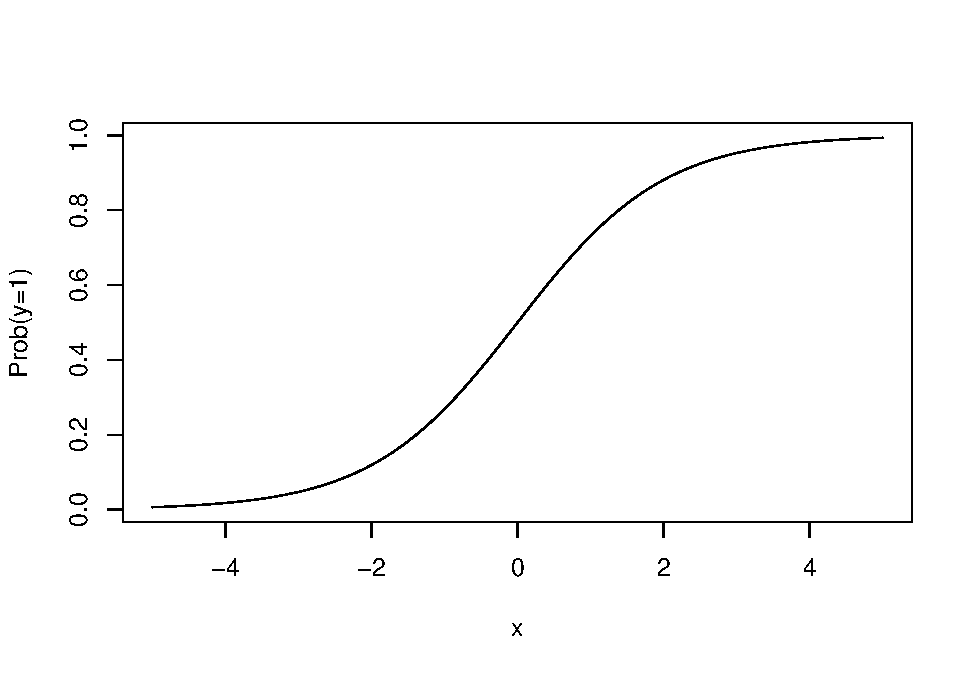
\includegraphics{classification1_files/figure-latex/unnamed-chunk-9-1.pdf}

Notice how we substituted \texttt{inv.logit()} to \texttt{plogis()} but
the output is the same. \texttt{plogis} is R's built in method that
return a logistic distribution function. \texttt{qlogis(p)} is exactly
the same as \texttt{logit(p)\ =\ log(p/(1-p))}, and \texttt{plogis(p)}
has consequently been called the ``inverse logit''.

Another important observation: realize that regardless of what value x
takes, our probability of success (y=1) will always be on the range of 0
to 1.

\hypertarget{key-assumptions-of-logistic-regression}{%
\subsection{Key Assumptions of Logistic
Regression}\label{key-assumptions-of-logistic-regression}}

Many of the key assumptions of linear regression do not hold true with
logistic regression. We've learned about the linearity assumption,
normality of residuals, and homoskedasticity assumptions in our
regression models class - they do not apply in the case of logistic
regression.

Logistic regression \textbf{does not} require a linear relationship
between the dependent and independent variables - it also does not
assume normality of residuals nor is it concerned with the problem of
heteroskedasticity the way that linear regressions are.

However, a few of the assumptions do apply:\\
- Multicollinearity: Just as with the case of linear regression,
logistic regression assumes little to no multicollinearity among the
independent variables (recall how we used VIF to identify highly
correlated variables in the last workshop)\\
- Independence of Observations: The observations should not come from
repeated measurements and are independent from each other\\
- Linearity of predictor and log odds: While logistic regressions do not
assume linearity between the dependent and independent variables, it
does assume that the independent variables (predictors) are linearly
related to the log odds.

The first two points are rather self-explanatory, and the third will be
illustrated to you in an example later (flight delay prediction). If put
slightly differently, the third point stresses that a logistic
regression models the logit-transformed probability as a linear
relationship with the predictor variables.

\hypertarget{binary-logistic-regression}{%
\subsection{Binary Logistic
Regression}\label{binary-logistic-regression}}

Supposed you work in an education institution and are put in charge to
evaluate the likelihood of a student graduating with a honors degree
given their academic scores in a reading test, writing test and
mathematics test.

This dataset has four features: \texttt{female}, \texttt{read},
\texttt{write}, \texttt{math} and the target variable is \texttt{hon}, a
binary feature with 1 indicating that the student is in fact in an
honors class and 0 indicating otherwise. The dataset is credited to the
UCLA: Statistical Consulting Group (see credits for link and details).

\begin{Shaded}
\begin{Highlighting}[]
\NormalTok{honors }\OtherTok{\textless{}{-}} \FunctionTok{read.csv}\NormalTok{(}\StringTok{"data\_input/sample.csv"}\NormalTok{)}
\NormalTok{honors}\SpecialCharTok{$}\NormalTok{hon }\OtherTok{\textless{}{-}} \FunctionTok{as.factor}\NormalTok{(honors}\SpecialCharTok{$}\NormalTok{hon)}
\FunctionTok{prop.table}\NormalTok{(}\FunctionTok{table}\NormalTok{(honors}\SpecialCharTok{$}\NormalTok{hon))}
\end{Highlighting}
\end{Shaded}

\begin{verbatim}
## 
##     0     1 
## 0.755 0.245
\end{verbatim}

In R, fitting a logistic regression is done using the \texttt{glm()}
function with the \texttt{family="binomial} parameter; To fully
understand logistic regression, let's begin by regressing \texttt{hon}
with no predictor variables.

\hypertarget{logistic-regression-with-no-predictor-variables}{%
\subsubsection{Logistic regression with no predictor
variables}\label{logistic-regression-with-no-predictor-variables}}

\begin{Shaded}
\begin{Highlighting}[]
\NormalTok{honors.logit }\OtherTok{\textless{}{-}} \FunctionTok{glm}\NormalTok{(hon }\SpecialCharTok{\textasciitilde{}} \DecValTok{1}\NormalTok{, }\AttributeTok{data=}\NormalTok{honors, }\AttributeTok{family=}\StringTok{"binomial"}\NormalTok{) }
\FunctionTok{summary}\NormalTok{(honors.logit)}
\end{Highlighting}
\end{Shaded}

\begin{verbatim}
## 
## Call:
## glm(formula = hon ~ 1, family = "binomial", data = honors)
## 
## Deviance Residuals: 
##     Min       1Q   Median       3Q      Max  
## -0.7497  -0.7497  -0.7497  -0.7497   1.6772  
## 
## Coefficients:
##             Estimate Std. Error z value         Pr(>|z|)    
## (Intercept)  -1.1255     0.1644  -6.845 0.00000000000762 ***
## ---
## Signif. codes:  0 '***' 0.001 '**' 0.01 '*' 0.05 '.' 0.1 ' ' 1
## 
## (Dispersion parameter for binomial family taken to be 1)
## 
##     Null deviance: 222.71  on 199  degrees of freedom
## Residual deviance: 222.71  on 199  degrees of freedom
## AIC: 224.71
## 
## Number of Fisher Scoring iterations: 4
\end{verbatim}

Recall from the earlier section that our \texttt{logit()} function,
formally defined, is expressed as:\\
\(y = log(\frac{p}{1-p})\) where \(p = \frac{x - min}{max-min}\)

\begin{Shaded}
\begin{Highlighting}[]
\FunctionTok{table}\NormalTok{(honors}\SpecialCharTok{$}\NormalTok{hon)}
\end{Highlighting}
\end{Shaded}

\begin{verbatim}
## 
##   0   1 
## 151  49
\end{verbatim}

P(honors) = 49/200 p(!honors) = 151/200

\begin{Shaded}
\begin{Highlighting}[]
\FunctionTok{log}\NormalTok{((}\DecValTok{49}\SpecialCharTok{/}\DecValTok{200}\NormalTok{)}\SpecialCharTok{/}\NormalTok{(}\DecValTok{151}\SpecialCharTok{/}\DecValTok{200}\NormalTok{))}
\end{Highlighting}
\end{Shaded}

\begin{verbatim}
## [1] -1.12546
\end{verbatim}

Our odds ratio, without the influence of any predictor variable, is 49
out of 200 (49 in honors classes vs 151 not), so that give us a
probability of 49/200, p = 0.245. Our odds ratio is therefore
0.245/(1-0.245) = 0.3245033

Taking the log of 0.3245033, our log of odds is therefore:

\begin{Shaded}
\begin{Highlighting}[]
\FunctionTok{log}\NormalTok{(}\FloatTok{0.3245033}\NormalTok{)}
\end{Highlighting}
\end{Shaded}

\begin{verbatim}
## [1] -1.12546
\end{verbatim}

This is essentially what our logistic regression model gave us:

\begin{Shaded}
\begin{Highlighting}[]
\FunctionTok{coefficients}\NormalTok{(honors.logit)}
\end{Highlighting}
\end{Shaded}

\begin{verbatim}
## (Intercept) 
##    -1.12546
\end{verbatim}

Observe how, when we take \textbf{log(p/(1-p))} or \textbf{log(odds
ratio)}, we find the same value of -1.12546, confirming our
understanding that the log of odds is the intercept from the model
without any predictor variables.

If we have wanted the log of odds in the form of probability, we could
do that too:

\begin{Shaded}
\begin{Highlighting}[]
\FunctionTok{exp}\NormalTok{(}\SpecialCharTok{{-}}\FloatTok{1.12546}\NormalTok{)}\SpecialCharTok{/}\NormalTok{(}\DecValTok{1}\SpecialCharTok{+}\FunctionTok{exp}\NormalTok{(}\SpecialCharTok{{-}}\FloatTok{1.12546}\NormalTok{))}
\end{Highlighting}
\end{Shaded}

\begin{verbatim}
## [1] 0.2449999
\end{verbatim}

And\ldots{} that's 0.245, which is the equivalent of 49/200 (probability
of success!)

If you need a refresher, recall that:\\
\(p = \frac{e^z}{1+e^z}\) Or scroll back to line 200 to look at the
mathematical details of the logit function.

\hypertarget{logistic-regression-with-one-discrete-predictor-variable}{%
\subsubsection{Logistic regression with one discrete predictor
variable}\label{logistic-regression-with-one-discrete-predictor-variable}}

Let's now add one binary predictor variable, \textbf{female} to the
model, such that the equation for our model is formally described as:
\(logit(p) = \beta_0 + \beta_1 * female\)

\begin{Shaded}
\begin{Highlighting}[]
\NormalTok{honors.logit2 }\OtherTok{\textless{}{-}} \FunctionTok{glm}\NormalTok{(hon }\SpecialCharTok{\textasciitilde{}}\NormalTok{ female, }\AttributeTok{data=}\NormalTok{honors, }\AttributeTok{family=}\StringTok{"binomial"}\NormalTok{)}
\end{Highlighting}
\end{Shaded}

Before we attempt to interpret the parameters estimated from our model
above, let's examine the odds ratio of a female being in a honors class
as we did before:

\begin{Shaded}
\begin{Highlighting}[]
\FunctionTok{table}\NormalTok{(}\AttributeTok{honors =}\NormalTok{ honors}\SpecialCharTok{$}\NormalTok{hon, }\AttributeTok{female =}\NormalTok{ honors}\SpecialCharTok{$}\NormalTok{female)}
\end{Highlighting}
\end{Shaded}

\begin{verbatim}
##       female
## honors  0  1
##      0 74 77
##      1 17 32
\end{verbatim}

\begin{itemize}
\tightlist
\item
  For males: odds of being in honors class = (17/91)/(74/91) =
  0.2297297\\
\item
  For females: odds of being in honors class = (32/109)/(77/109) =
  0.4155844\\
\item
  The ratio of the odds for female vs ratio of the odds for male =
  .42/.23 = 1.809, which is to say that the odds for female being in an
  honors class are about 81\% more than that of their male counterpart
\end{itemize}

\begin{Shaded}
\begin{Highlighting}[]
\FunctionTok{paste}\NormalTok{(}\StringTok{"Male:"}\NormalTok{, (}\DecValTok{17}\SpecialCharTok{/}\DecValTok{91}\NormalTok{)}\SpecialCharTok{/}\NormalTok{(}\DecValTok{74}\SpecialCharTok{/}\DecValTok{91}\NormalTok{))}
\end{Highlighting}
\end{Shaded}

\begin{verbatim}
## [1] "Male: 0.22972972972973"
\end{verbatim}

\begin{Shaded}
\begin{Highlighting}[]
\FunctionTok{paste}\NormalTok{(}\StringTok{"Female:"}\NormalTok{, (}\DecValTok{32}\SpecialCharTok{/}\DecValTok{109}\NormalTok{)}\SpecialCharTok{/}\NormalTok{(}\DecValTok{77}\SpecialCharTok{/}\DecValTok{109}\NormalTok{))}
\end{Highlighting}
\end{Shaded}

\begin{verbatim}
## [1] "Female: 0.415584415584416"
\end{verbatim}

Getting the log of odds:

\begin{Shaded}
\begin{Highlighting}[]
\CommentTok{\#log(odds ratio)}
\FunctionTok{log}\NormalTok{(}\FloatTok{0.4155844}\SpecialCharTok{/}\FloatTok{0.2297297}\NormalTok{)}
\end{Highlighting}
\end{Shaded}

\begin{verbatim}
## [1] 0.5927823
\end{verbatim}

Let's now relate the odds ratio to the output from the logistic
regression model with our \texttt{female} predictor variable.

\begin{Shaded}
\begin{Highlighting}[]
\FunctionTok{summary}\NormalTok{(honors.logit2)}
\end{Highlighting}
\end{Shaded}

\begin{verbatim}
## 
## Call:
## glm(formula = hon ~ female, family = "binomial", data = honors)
## 
## Deviance Residuals: 
##     Min       1Q   Median       3Q      Max  
## -0.8337  -0.8337  -0.6431  -0.6431   1.8317  
## 
## Coefficients:
##             Estimate Std. Error z value     Pr(>|z|)    
## (Intercept)  -1.4709     0.2690  -5.469 0.0000000453 ***
## female        0.5928     0.3414   1.736       0.0825 .  
## ---
## Signif. codes:  0 '***' 0.001 '**' 0.01 '*' 0.05 '.' 0.1 ' ' 1
## 
## (Dispersion parameter for binomial family taken to be 1)
## 
##     Null deviance: 222.71  on 199  degrees of freedom
## Residual deviance: 219.61  on 198  degrees of freedom
## AIC: 223.61
## 
## Number of Fisher Scoring iterations: 4
\end{verbatim}

The intercept of \textbf{-1.4709} is the log odds for males since male
is the reference group (\textbf{female} = 0). If we have wanted to
confirm this, we can manually calculate this using the odds ratio for
the male group:

\begin{Shaded}
\begin{Highlighting}[]
\FunctionTok{log}\NormalTok{(}\FloatTok{0.2297297}\NormalTok{)}
\end{Highlighting}
\end{Shaded}

\begin{verbatim}
## [1] -1.470852
\end{verbatim}

The coefficient for \textbf{female} is the log of odds ratio between the
female group and the male group, which can be manually calculated:

\begin{Shaded}
\begin{Highlighting}[]
\FunctionTok{log}\NormalTok{(}\FloatTok{1.809}\NormalTok{)}
\end{Highlighting}
\end{Shaded}

\begin{verbatim}
## [1] 0.5927742
\end{verbatim}

Using what we've learned earlier, we also know how easy it would be for
us to calculate the odds ratio from the output of the model's summary:
we simply have to exponentiate the coefficient it gives us for female.

And if we were to relate this back to the original equation:
\(logit(p) = \beta_0 + \beta_1 * female\)

\begin{itemize}
\tightlist
\item
  For a male (female = 0): we would substitute the values into the
  equation and arrive at logit(p) = -1.4709\\
\item
  For a female (female = 1): we would instead get logit(p) = -1.4709 +
  (0.5928*1) = -0.8781
\end{itemize}

\begin{Shaded}
\begin{Highlighting}[]
\CommentTok{\# calculating the change in odds}
\CommentTok{\# odds of female in honors / odds of male in honors}
\CommentTok{\# log of odds to odds is an exponent transformation}
\FunctionTok{exp}\NormalTok{(}\SpecialCharTok{{-}}\FloatTok{0.8781}\NormalTok{)}\SpecialCharTok{/}\FunctionTok{exp}\NormalTok{(}\SpecialCharTok{{-}}\FloatTok{1.4709}\NormalTok{)}
\end{Highlighting}
\end{Shaded}

\begin{verbatim}
## [1] 1.809047
\end{verbatim}

\begin{quote}
The ratio of the odds for female vs ratio of the odds for male = .42/.23
= 1.809, which is to say that the odds for female being in an honors
class are about 81\% more than that of their male counterpart
\end{quote}

Notice how this is the same answer we derive from our manual calculation
even before looking at the output of our logistic regression model. In
fact, we could as well have taken the \textbf{estimated coefficient}
value for \texttt{female}, which the output says is 0.5928, and get its
exponent:

\begin{Shaded}
\begin{Highlighting}[]
\FunctionTok{exp}\NormalTok{(honors.logit2}\SpecialCharTok{$}\NormalTok{coefficients[}\StringTok{"female"}\NormalTok{])}
\end{Highlighting}
\end{Shaded}

\begin{verbatim}
##   female 
## 1.809015
\end{verbatim}

\hypertarget{logistic-regression-with-one-continuous-predictor-variable}{%
\subsubsection{Logistic regression with one continuous predictor
variable}\label{logistic-regression-with-one-continuous-predictor-variable}}

Let's try another exercise, this time using the \texttt{math} score
(continuous variable) such that the equation for our model is formally
described as: \(logit(p) = \beta_0 + \beta_1 * math\)

\begin{Shaded}
\begin{Highlighting}[]
\NormalTok{honors.logit3 }\OtherTok{\textless{}{-}} \FunctionTok{glm}\NormalTok{( hon }\SpecialCharTok{\textasciitilde{}}\NormalTok{ math, }\AttributeTok{data=}\NormalTok{honors, }\AttributeTok{family=}\StringTok{"binomial"}\NormalTok{ )}
\FunctionTok{summary}\NormalTok{(honors.logit3)}
\end{Highlighting}
\end{Shaded}

\begin{verbatim}
## 
## Call:
## glm(formula = hon ~ math, family = "binomial", data = honors)
## 
## Deviance Residuals: 
##     Min       1Q   Median       3Q      Max  
## -2.0332  -0.6785  -0.3506  -0.1565   2.6143  
## 
## Coefficients:
##             Estimate Std. Error z value        Pr(>|z|)    
## (Intercept) -9.79394    1.48174  -6.610 0.0000000000385 ***
## math         0.15634    0.02561   6.105 0.0000000010294 ***
## ---
## Signif. codes:  0 '***' 0.001 '**' 0.01 '*' 0.05 '.' 0.1 ' ' 1
## 
## (Dispersion parameter for binomial family taken to be 1)
## 
##     Null deviance: 222.71  on 199  degrees of freedom
## Residual deviance: 167.07  on 198  degrees of freedom
## AIC: 171.07
## 
## Number of Fisher Scoring iterations: 5
\end{verbatim}

Notice in the case of a continuous variable such as the math score, our
estimated coefficient for the intercept is the log-odds of a student
with a math score of zero being in an honors class. If we mentally
visualize a plot with both x and y axis, this makes intuitive sense: the
intercept points to the value of y \textbf{when our x feature = 0}. By
taking the exponent of this value, we can then know the odds of such
student being in an honors class:

\begin{Shaded}
\begin{Highlighting}[]
\FunctionTok{exp}\NormalTok{(honors.logit3}\SpecialCharTok{$}\NormalTok{coefficients[}\StringTok{"(Intercept)"}\NormalTok{])}
\end{Highlighting}
\end{Shaded}

\begin{verbatim}
##   (Intercept) 
## 0.00005578854
\end{verbatim}

These odds are very low, and a peek at the distribution for the variable
math will reveal that no one in the sample has a math score lower than
30 (mean of 53 in fact), which tells us that the intercept in this model
corresponds to the log odds of being in an honors class when math is at
the hypothetical value of zero.

How do we interpret the coefficient for math? Recall our equation:
\(logit(p) = log(p/(1-p)) = \beta_0 + \beta_1 * math\)

With the substituted values: logit(p) = -9.79394 + 0.15634 * math

\begin{Shaded}
\begin{Highlighting}[]
\FunctionTok{hist}\NormalTok{(honors}\SpecialCharTok{$}\NormalTok{math, }\AttributeTok{breaks=}\DecValTok{20}\NormalTok{)}
\FunctionTok{abline}\NormalTok{(}\AttributeTok{v=}\FunctionTok{median}\NormalTok{(honors}\SpecialCharTok{$}\NormalTok{math), }\AttributeTok{col=}\StringTok{"blue"}\NormalTok{, }\AttributeTok{lwd=}\DecValTok{3}\NormalTok{)}
\end{Highlighting}
\end{Shaded}

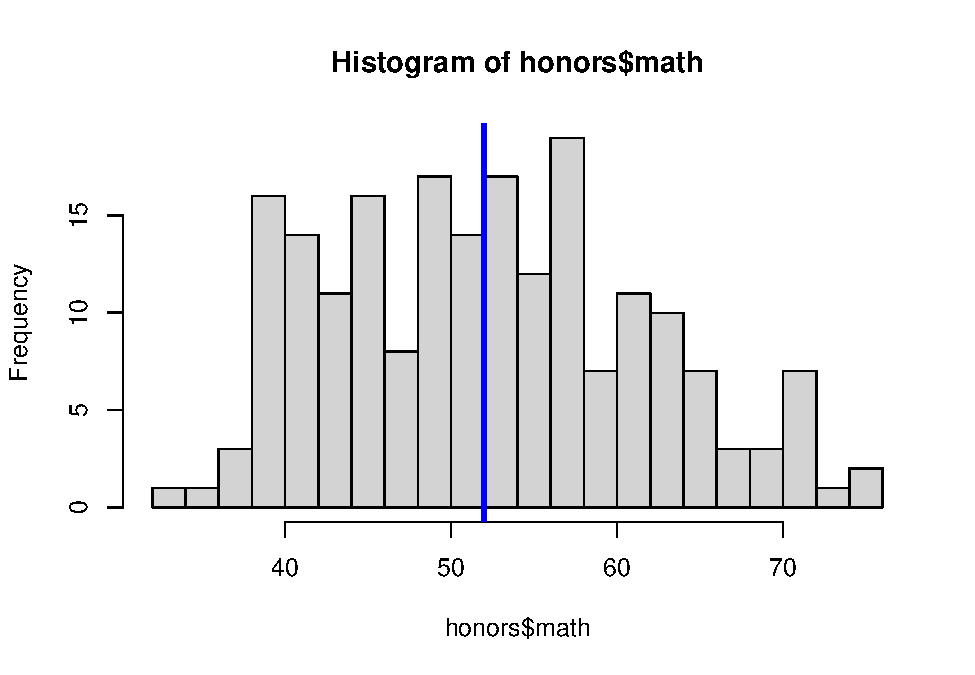
\includegraphics{classification1_files/figure-latex/unnamed-chunk-28-1.pdf}

The median of math is \textasciitilde52. Let's assume a \texttt{math}
value of 52: logit(p) = -9.79394 + 0.15634 * 52 = -1.66426

Examine the effect of a one-unit increase in math score, at 53: logit(p)
= -9.79394 + 0.15634 * 53 = -1.50792

Taking the difference: -1.50792 - (-1.66426) = 0.15634

\begin{Shaded}
\begin{Highlighting}[]
\SpecialCharTok{{-}}\FloatTok{1.50792} \SpecialCharTok{{-}}\NormalTok{ (}\SpecialCharTok{{-}}\FloatTok{1.66426}\NormalTok{)}
\end{Highlighting}
\end{Shaded}

\begin{verbatim}
## [1] 0.15634
\end{verbatim}

\begin{Shaded}
\begin{Highlighting}[]
\CommentTok{\# 0.15634, the diff with a one{-}unit increase should also be the}
\CommentTok{\# coefficient for our math variable}
\NormalTok{honors.logit3}\SpecialCharTok{$}\NormalTok{coefficients[}\DecValTok{2}\NormalTok{]}
\end{Highlighting}
\end{Shaded}

\begin{verbatim}
##      math 
## 0.1563404
\end{verbatim}

\ldots and that checks out with our manual calculation! So the
coefficient for \texttt{math} is in fact the difference in the log odds
for one unit of increment in that variable (math score of 53 vs 52). In
simpler words, for one-unit increase in the math score, the expected
change in log odds is 0.15634.

Like the earlier example, we could also translate this change in log
odds to the change in odds by exponentiating the log-odds:

Change in Odds = odds(math=53) / odds(math=52)\\
= exp(-1.50792) / exp(-1.66426)\\
= odds (difference in one-unit increase)\\
= exp(0.15634)\\
= 1.169224

\begin{Shaded}
\begin{Highlighting}[]
\FunctionTok{exp}\NormalTok{(}\SpecialCharTok{{-}}\FloatTok{1.50792}\NormalTok{) }\SpecialCharTok{/} \FunctionTok{exp}\NormalTok{(}\SpecialCharTok{{-}}\FloatTok{1.66426}\NormalTok{)}
\end{Highlighting}
\end{Shaded}

\begin{verbatim}
## [1] 1.169224
\end{verbatim}

\begin{Shaded}
\begin{Highlighting}[]
\FunctionTok{exp}\NormalTok{(}\SpecialCharTok{{-}}\FloatTok{1.50792} \SpecialCharTok{{-}} \SpecialCharTok{{-}}\FloatTok{1.66426}\NormalTok{)}
\end{Highlighting}
\end{Shaded}

\begin{verbatim}
## [1] 1.169224
\end{verbatim}

\begin{Shaded}
\begin{Highlighting}[]
\FunctionTok{exp}\NormalTok{(}\FloatTok{0.15634}\NormalTok{)}
\end{Highlighting}
\end{Shaded}

\begin{verbatim}
## [1] 1.169224
\end{verbatim}

\begin{Shaded}
\begin{Highlighting}[]
\FunctionTok{exp}\NormalTok{(honors.logit3}\SpecialCharTok{$}\NormalTok{coefficients[}\DecValTok{2}\NormalTok{])}
\end{Highlighting}
\end{Shaded}

\begin{verbatim}
##     math 
## 1.169224
\end{verbatim}

We interpret this as: for a one-unit increase in math score, we expect
to see \textasciitilde17\% increase in the odds of being in an honors
class. This 17\% does not depend on the value that math is held at. It's
also important to note that a 17\% increase in odds is not the same as a
17\% increase in probability. All it is saying that compared to a score
of 52, scoring 53 will improve the odds of being in an honors class by
1.17 times.

\hypertarget{logistic-regression-with-multiple-predictor-variables-and-no-interaction-terms}{%
\subsubsection{Logistic regression with multiple predictor variables and
no interaction
terms}\label{logistic-regression-with-multiple-predictor-variables-and-no-interaction-terms}}

In general, we can have multiple predictor variables in a logistic
regression model: logit(p) = log(p/(1-p))\\
= \(\beta_0 + \beta1 * x1 + ... + \beta_k *xk\)

Applying such a model to our example dataset, each estimated coefficient
is the expected change in the log odds of being in an honors class
\textbf{for a one-unit increase in the corresponding predictor variable}
holding the other variables constant at a certain value. Each
exponentiated coefficient is the ratio of two odds, or the change in
odds in the multiplicative scale for a one-unit increase in the
corresponding predictor variable holding other variables at a certain
value. Let's look at the following equation:

\(logit(p) = \beta_0 + \beta_1 * math + \beta_2 * female + \beta_3 * read\)

\begin{Shaded}
\begin{Highlighting}[]
\NormalTok{honors.logit4 }\OtherTok{\textless{}{-}} \FunctionTok{glm}\NormalTok{(hon }\SpecialCharTok{\textasciitilde{}}\NormalTok{ math }\SpecialCharTok{+}\NormalTok{ female }\SpecialCharTok{+}\NormalTok{ read, }\AttributeTok{data=}\NormalTok{honors, }\AttributeTok{family=}\StringTok{"binomial"}\NormalTok{)}
\FunctionTok{summary}\NormalTok{(honors.logit4)}
\end{Highlighting}
\end{Shaded}

\begin{verbatim}
## 
## Call:
## glm(formula = hon ~ math + female + read, family = "binomial", 
##     data = honors)
## 
## Deviance Residuals: 
##     Min       1Q   Median       3Q      Max  
## -1.8305  -0.6327  -0.3300  -0.1258   2.3896  
## 
## Coefficients:
##              Estimate Std. Error z value         Pr(>|z|)    
## (Intercept) -11.77025    1.71068  -6.880 0.00000000000597 ***
## math          0.12296    0.03128   3.931 0.00008442731719 ***
## female        0.97995    0.42163   2.324           0.0201 *  
## read          0.05906    0.02655   2.224           0.0261 *  
## ---
## Signif. codes:  0 '***' 0.001 '**' 0.01 '*' 0.05 '.' 0.1 ' ' 1
## 
## (Dispersion parameter for binomial family taken to be 1)
## 
##     Null deviance: 222.71  on 199  degrees of freedom
## Residual deviance: 156.17  on 196  degrees of freedom
## AIC: 164.17
## 
## Number of Fisher Scoring iterations: 5
\end{verbatim}

The coefficient for \emph{math} tells us that, holding \emph{female} and
\emph{reading} at a fixed value (``constant''), we will see a 13\%
increase in the odds of graduating with honors class for a one-unit
increase in math score since exp(.12296) = 1.13.

As a warm-up to your graded assignment (for full Academy students), can
you attempt to interpret the above model and answer the following
question?

\begin{itemize}
\tightlist
\item
  Holding Female and Mathematics score constant, a one-unit increase in
  reading score improves the odds of graduating with honors by how much?
\end{itemize}

\begin{Shaded}
\begin{Highlighting}[]
\FunctionTok{exp}\NormalTok{(}\FloatTok{0.05906}\NormalTok{)}
\end{Highlighting}
\end{Shaded}

\begin{verbatim}
## [1] 1.060839
\end{verbatim}

\hypertarget{extra-example-predicting-flight-delay}{%
\subsubsection{Extra Example: Predicting Flight
Delay}\label{extra-example-predicting-flight-delay}}

Let's take a look at what happened when we try to predict flight delays
using a logistic regression models where the predictor variables are
\texttt{Month}, \texttt{DayofMonth}, and \texttt{DayofWeek}
respectively.

\begin{Shaded}
\begin{Highlighting}[]
\NormalTok{flights.s }\OtherTok{\textless{}{-}} \FunctionTok{read.csv}\NormalTok{(}\StringTok{"data\_input/flight\_sm.csv"}\NormalTok{)}

\FunctionTok{summary}\NormalTok{(}\FunctionTok{glm}\NormalTok{(DepDel15 }\SpecialCharTok{\textasciitilde{}}\NormalTok{ Month }\SpecialCharTok{+}\NormalTok{ DayofMonth }\SpecialCharTok{+}\NormalTok{ DayofWeek, }\AttributeTok{data=}\NormalTok{flights.s, }\AttributeTok{family=}\StringTok{"binomial"}\NormalTok{))}
\end{Highlighting}
\end{Shaded}

\begin{verbatim}
## 
## Call:
## glm(formula = DepDel15 ~ Month + DayofMonth + DayofWeek, family = "binomial", 
##     data = flights.s)
## 
## Deviance Residuals: 
##     Min       1Q   Median       3Q      Max  
## -0.7421  -0.6941  -0.6531  -0.6144   1.8902  
## 
## Coefficients:
##               Estimate Std. Error z value             Pr(>|z|)    
## (Intercept) -0.9747469  0.0150960 -64.570 < 0.0000000000000002 ***
## Month       -0.0610039  0.0017178 -35.512 < 0.0000000000000002 ***
## DayofMonth   0.0025760  0.0003863   6.668      0.0000000000259 ***
## DayofWeek   -0.0048308  0.0017104  -2.824              0.00474 ** 
## ---
## Signif. codes:  0 '***' 0.001 '**' 0.01 '*' 0.05 '.' 0.1 ' ' 1
## 
## (Dispersion parameter for binomial family taken to be 1)
## 
##     Null deviance: 541635  on 538362  degrees of freedom
## Residual deviance: 540321  on 538359  degrees of freedom
## AIC: 540329
## 
## Number of Fisher Scoring iterations: 4
\end{verbatim}

There is a problem with the above logistic regression model: Can you
tell which among the three key assumptions did it violate(s)? -
Multicollinearity\\
- Independence of Observations\\
- Linearity of predictor and log odds

\hypertarget{application-of-logistic-regression}{%
\subsection{Application of Logistic
Regression}\label{application-of-logistic-regression}}

In the field of market research where its commonplace for business
analysts to try and get as accurate as possible a prediction of a new
product launch (success/failure), a new bundle pricing strategy (odds of
success / odds of failure), or a new enrollment plan, logistic
regression and its accompanying analysis plays a pivotal role. An
example of this is the scenario of a company that is estimating the
change of probability / odds of customer buy-in for every \$1 dollar
change in price. Another example of this is in election forecasts: where
a campaign manager is trying to determine the odds of a likely voter to
vote for a particular candidate, using demographic parameters such as
gender, age, and education level.

Another common use of logistic regression in business is in building
models of customer retention, which can offer incredible insights into
why some customers leave and others stay (drivers of customer
retention). This is particularly important in certain industries, where
reducing customer defections by as little as five percent can double
profits (Reichheld, 1996\footnote{\href{}{Reichheld, F.F. (1996).,
  Learning from Customer Defections, in Harvard Business
  Review,march-april.}})

Another interest project that models customer retention using historical
data from a database (more than 500,000 clients) of a big mutual fund
investment company and logistic regression (Eiben, Euverman, Kowalczyk,
Slisser\footnote{\href{http://citeseerx.ist.psu.edu/viewdoc/download?doi=10.1.1.55.7177\&rep=rep1\&type=pdf}{Modelling
  Customer Retention with Statistical Techniques, Rough Data Models, and
  Genetic Programming.}}) highlights the benefits of an interpretative
model like the one we obtain with logistic regression.

A third area of application for logistic regression models is in the
modeling of customer churn and attrition\footnote{\href{http://www.academicjournals.org/article/article1379926496_Oghojafor\%20et\%20al.pdf}{Modelling
  telecom customer attrition using logistic regression}}:

\begin{figure}
\centering
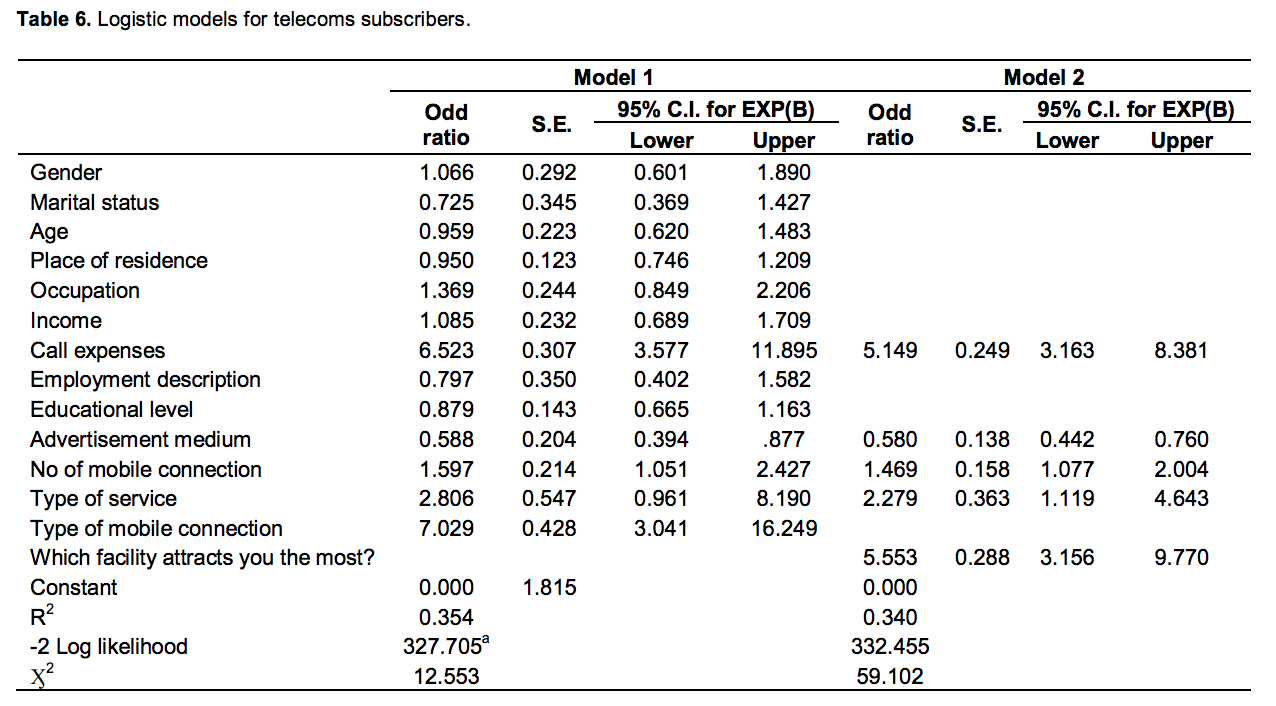
\includegraphics{assets/illustration1.png}
\caption{Investigating the effect of socio-economic factors on customer
attrition using logistic models}
\end{figure}

Yet another example is in Credit Risk Analysis, where machine learning
is deployed to estimate probability of loan defaults, or non-performing
loans (or in the measurement of other types of credit risk). The paper
described how loan officers at bank use logistic regression ``to
identify characteristics that are indicative of people who are likely to
default on loans, and then use those characteristics to discriminate
between good and bad credit risks''\footnote{\href{http://smartdrill.com/pdf/Credit\%20Risk\%20Analysis.pdf}{Credit
  Risk Analysis Using Logistic Regression Modeling}}.

A quick summary of the findings:\\
- Number of years at current employment and number of years at current
address have negative coefficients, indicating that customers who have
spent less time at either their current employer or their current
address are more likely to default\\
- Debt-to-income ratio (\texttt{dti}, a measurement we'll use in our
project later) and amount of credit card debt both have positive
coefficients, indicating that higher dti ratios or higher amounts of
credit card debts are both associated with a greater likelihood of loan
defaults.

\hypertarget{credit-risk-analysis-modeling-loans-from-q4-2017}{%
\subsection{Credit Risk Analysis / Modeling: Loans from Q4
2017}\label{credit-risk-analysis-modeling-loans-from-q4-2017}}

I've prepared the following data originally made available by
\href{https://www.lendingclub}{LendingClub}. Some preprocessing steps
have been applied to save you from the ``data cleansing'' work. We'll
read the data into our workspace:

\begin{Shaded}
\begin{Highlighting}[]
\NormalTok{loans.s }\OtherTok{\textless{}{-}} \FunctionTok{read.csv}\NormalTok{(}\StringTok{"data\_input/loan2017Q4.csv"}\NormalTok{)}
\FunctionTok{str}\NormalTok{(loans.s)}
\end{Highlighting}
\end{Shaded}

\begin{verbatim}
## 'data.frame':    1556 obs. of  16 variables:
##  $ initial_list_status: chr  "w" "f" "w" "w" ...
##  $ purpose            : chr  "debt_consolidation" "debt_consolidation" "debt_consolidation" "debt_consolidation" ...
##  $ int_rate           : num  14.08 9.44 28.72 13.59 15.05 ...
##  $ installment        : num  676 480 1010 484 476 ...
##  $ annual_inc         : num  156700 50000 25000 175000 109992 ...
##  $ dti                : num  19.1 19.4 65.6 12.6 10 ...
##  $ verification_status: chr  "Source Verified" "Not Verified" "Verified" "Not Verified" ...
##  $ grade              : chr  "C" "B" "F" "C" ...
##  $ revol_bal          : int  21936 5457 23453 31740 2284 2016 14330 27588 27024 11719 ...
##  $ inq_last_12m       : int  3 1 0 0 3 5 0 1 8 1 ...
##  $ delinq_2yrs        : int  0 1 0 0 0 0 0 0 0 0 ...
##  $ home_ownership     : chr  "MORTGAGE" "RENT" "OWN" "MORTGAGE" ...
##  $ not_paid           : int  0 1 1 1 0 1 0 1 1 0 ...
##  $ log_inc            : num  12 10.8 10.1 12.1 11.6 ...
##  $ verified           : int  1 0 1 0 0 0 0 0 1 1 ...
##  $ grdCtoA            : int  0 1 0 0 0 1 0 1 0 0 ...
\end{verbatim}

The variable of interest is the \texttt{not\_paid} variable, a binary
variable that indicate whether a loan is fully paid or not. A loan is
considered ``not paid'' (not paid = 1) when it is \textbf{Defaulted},
\textbf{Charged Off}, or past due date (\textbf{Grace Period}). To
prevent one class from dominating the other, the data I've prepared here
over-sampled more ``bad'' loans so that the underlying characteristics
of the empirically minority class is adequately represented.

\begin{Shaded}
\begin{Highlighting}[]
\FunctionTok{table}\NormalTok{(loans.s}\SpecialCharTok{$}\NormalTok{not\_paid)}
\end{Highlighting}
\end{Shaded}

\begin{verbatim}
## 
##   0   1 
## 778 778
\end{verbatim}

What's important to note is that logistic regression is not susceptible
to a ``class imbalance'' problem per-se, and an unbalanced class
representation is for the most part dealt with as sample size grows
anyway. That said, in the situation of highly imbalanced class
representation, the patterns within the minority class may not be
sufficiently ``described'' and in the case of an extreme imbalance you
may be better off using an ``anomaly detection'' approach than through a
classification approach.

In the Unsupervised Machine Learning workshop within the Machine
Learning Specialization, I will delve into the specific details of
anomaly detection algorithms with far greater depth so let's stay on
track and study the dataset we've just read into our environment:\\
- \texttt{initial\_list\_status}: Either \texttt{w} (whole) or
\texttt{f} (fractional). This variable indicates if the loan was a whole
loan or fractional loan. For background: Some institutional investors
have a preference to purchase loans in their entirety to obtain legal
and accounting treatment specific to their situation - with the added
benefit of ``instant funding'' to borrowers\\
- \texttt{purpose}: Simplified from the original data; One of:
\texttt{credit\_card}, \texttt{debt\_consolidation},
\texttt{home\_improvement}, \texttt{major\_purchase} and
\texttt{small\_business}\\
- \texttt{int\_rate}: Interest rate in percentages\\
- \texttt{installment}: Monthly payment owed by the borrower\\
- \texttt{annual\_inc}: Self-reported annual income provided by the
borrower / co-borrowers during application\\
- \texttt{dti}: A ratio of the borrower's total monthly debt payments on
his/her total obligations to the self-reported monthly income\\
- \texttt{verification\_status}: is the reported income verified, not
verified, or if the income source was verified\\
- \texttt{grade}: software-assigned loan grade\\
- \texttt{revol\_bal}: total credit revolving balance (in the case of
credit card, it refers to the portion of credit card spending that goes
unpaid at the end of a billing cycle)\\
- \texttt{inq\_last\_12m}: number of credit inquiries in the last 12
months\\
- \texttt{delinq\_2yrs}: number of 30+ days past-due incidences of
delinquency in the borrower's credit file for the past 2 years\\
- \texttt{home\_ownership}: one of \texttt{MORTGAGE}, \texttt{OWN} and
\texttt{RENT}\\
- \texttt{not\_paid}: 0 for fully-paid loans, 1 for charged-off,
past-due / grace period or defaulted\\
- \texttt{log\_inc}: log of \texttt{annual\_inc}\\
- \texttt{verified}: 0 for ``Not verified'' under
\texttt{verification\_status}, 1 otherwise\\
- \texttt{grdCtoA}: 1 for a \texttt{grade} of A, B or C, 0 otherwise

Before we dive into building our classification model, I'd like to
encourage you to spend some time on the ``exploratory phase''. This is
the phase where you investigate the relationships and discover rough
structures of the data. You can use \texttt{summary()}, or
\texttt{fivenum()}, or even \texttt{cor()} - take your time to write a
few more lines of code below this chunk and be curious about your data!

\begin{Shaded}
\begin{Highlighting}[]
\FunctionTok{summary}\NormalTok{(loans.s[loans.s}\SpecialCharTok{$}\NormalTok{not\_paid }\SpecialCharTok{==} \DecValTok{0}\NormalTok{, }\StringTok{"dti"}\NormalTok{])}
\end{Highlighting}
\end{Shaded}

\begin{verbatim}
##    Min. 1st Qu.  Median    Mean 3rd Qu.    Max. 
##    0.00   11.02   16.82   18.34   23.79  198.56
\end{verbatim}

\begin{Shaded}
\begin{Highlighting}[]
\FunctionTok{summary}\NormalTok{(loans.s[loans.s}\SpecialCharTok{$}\NormalTok{not\_paid }\SpecialCharTok{==} \DecValTok{1}\NormalTok{, }\StringTok{"dti"}\NormalTok{])}
\end{Highlighting}
\end{Shaded}

\begin{verbatim}
##    Min. 1st Qu.  Median    Mean 3rd Qu.    Max. 
##    0.00   10.93   17.54   19.38   25.05  115.85
\end{verbatim}

\begin{Shaded}
\begin{Highlighting}[]
\FunctionTok{xtabs}\NormalTok{(dti }\SpecialCharTok{\textasciitilde{}}\NormalTok{ purpose }\SpecialCharTok{+}\NormalTok{ not\_paid, loans.s)}
\end{Highlighting}
\end{Shaded}

\begin{verbatim}
##                     not_paid
## purpose                     0        1
##   credit_card         3071.43  2830.58
##   debt_consolidation  9330.06 10127.08
##   home_improvement    1460.39  1386.24
##   major_purchase       170.15   476.46
##   small_business       237.94   256.14
\end{verbatim}

\begin{Shaded}
\begin{Highlighting}[]
\FunctionTok{plot}\NormalTok{(}\FunctionTok{xtabs}\NormalTok{(dti }\SpecialCharTok{\textasciitilde{}}\NormalTok{ grade }\SpecialCharTok{+}\NormalTok{ not\_paid, loans.s), }
     \AttributeTok{main=}\StringTok{"Assigned Grade of Loan vs Default"}\NormalTok{)}
\end{Highlighting}
\end{Shaded}

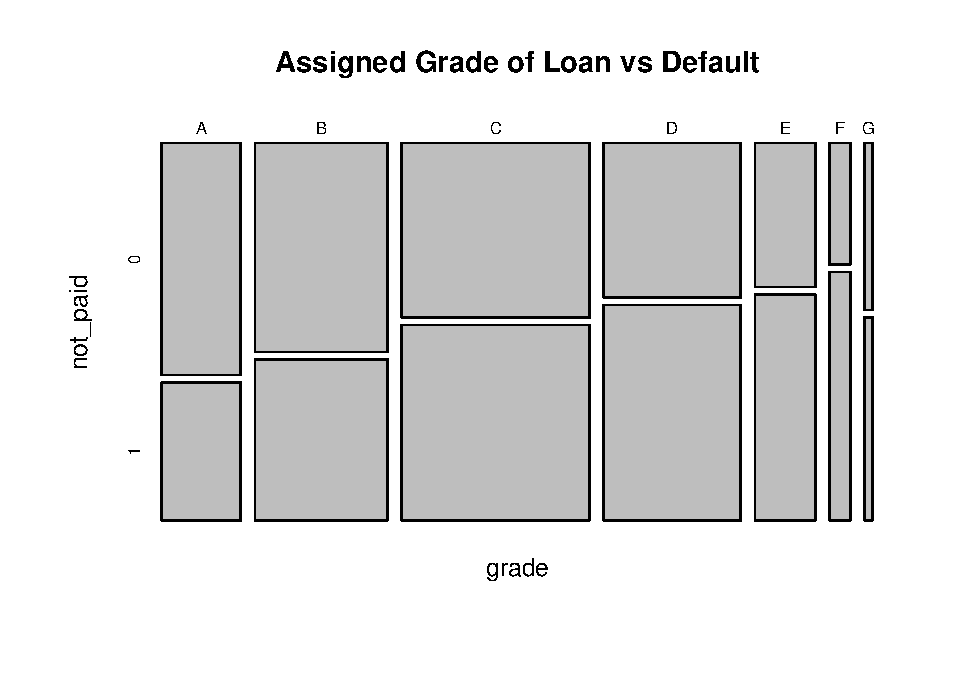
\includegraphics{classification1_files/figure-latex/unnamed-chunk-38-1.pdf}

\hypertarget{cross-validation-and-out-of-sample-error}{%
\subsubsection{Cross-Validation and Out-of-Sample
Error}\label{cross-validation-and-out-of-sample-error}}

Before we develop our classification model, I'll introduce you to the
idea of estimating the accuracy of our model. Simply put, we are going
to:\\
- Split our dataset into train and test sets\\
- Build our machine learning model using data \textbf{only} from our
train set\\
- Obtain an unbiased measurement of the model's accuracy by predicting
on test set

A related idea is known as \textbf{cross-validation}, in which we:\\
- Split our dataset into train, cross-validation, and test sets\\
- Develop the initial model using our train set\\
- Evaluate model on cross-validation set(s), returning to the previous
step if necessary (say, pick different predictor variables, use a
different parameter, or to tune other aspects of the model
specification)\\
- Pick a final model based on an evaluation criteria (Adj.R-squared,
accuracy, etc)\\
- Obtain an unbiased measurement of the model's accuracy by predicting
on test set

We can repeat step(2) and step(3) as much as is necessary, testing out
different algorithms or model specification, or combinations of
predictor variables and pick a final model on which we will obtain our
estimated accuracy by testing it on the test set. An important rule on
this is that the \textbf{test set must not be used in any of the steps
before the (5)}, such that the accuracy we obtain is an unbiased
measurement of the out-of-sample accuracy of the model.

The idea of obtaining an unbiased estimate of our model's out-of-sample
performance is an important one as it is often the case that the
in-sample error (the error you obtain from running your algorithm on the
dataset it was trained on) is optimistic and tuned / adapted in a
particular way to minimize the error in the training sample. Therefore -
the in-sample error is not a good representation or indication of how
our model will perform when it is applied on unseen data.

Another way to think about is that our training data has two components
to it: signal and noise. The goal of machine learning is to identify the
signal but be robust enough to avoid modeling the ``noise'' component of
the data. When we build a model, we want to know that our model is not
overly adapted to the data set to the point that it captures both the
signal and noise, a phenomenon known as ``overfitting''. When our model
is guilty of overfitting, the in-sample accuracy will be very high (in
some cases \textasciitilde100\%) but fail to perform on unseen data. The
idea is to strike the right balance between accuracy (don't underfit)
and robustness to noise (don't overfit).

\hypertarget{predicting-credit-risk-from-loans}{%
\subsubsection{Predicting Credit Risk from
Loans}\label{predicting-credit-risk-from-loans}}

Applying what we've learned above, we'll split our data into the
\texttt{loans.train} and \texttt{loans.test} set. I'll first show you
this approach and later show you the cross-validation approach - I
encourage you to follow this part of the workshop closely:

\begin{Shaded}
\begin{Highlighting}[]
\FunctionTok{RNGkind}\NormalTok{(}\AttributeTok{sample.kind=}\StringTok{"Rounding"}\NormalTok{)}
\end{Highlighting}
\end{Shaded}

\begin{verbatim}
## Warning in RNGkind(sample.kind = "Rounding"): non-uniform 'Rounding' sampler
## used
\end{verbatim}

\begin{Shaded}
\begin{Highlighting}[]
\FunctionTok{set.seed}\NormalTok{(}\DecValTok{417}\NormalTok{)}
\NormalTok{intrain }\OtherTok{\textless{}{-}} \FunctionTok{sample}\NormalTok{(}\FunctionTok{nrow}\NormalTok{(loans.s), }\FunctionTok{nrow}\NormalTok{(loans.s)}\SpecialCharTok{*}\FloatTok{0.8}\NormalTok{)}
\NormalTok{loans.train }\OtherTok{\textless{}{-}}\NormalTok{ loans.s[intrain, ]}
\NormalTok{loans.test }\OtherTok{\textless{}{-}}\NormalTok{ loans.s[}\SpecialCharTok{{-}}\NormalTok{intrain, ]}
\end{Highlighting}
\end{Shaded}

We already know how to build a binomial logistic regression and learned
the ``manual'' way of obtaining those coefficients in previous sections.
Here we'll cut to the chase and use \texttt{glm} for our model
construction:

\begin{Shaded}
\begin{Highlighting}[]
\NormalTok{creditrisk }\OtherTok{\textless{}{-}} \FunctionTok{glm}\NormalTok{(not\_paid }\SpecialCharTok{\textasciitilde{}}\NormalTok{ verified }\SpecialCharTok{+}\NormalTok{ purpose }\SpecialCharTok{+}\NormalTok{ installment }\SpecialCharTok{+}\NormalTok{ int\_rate }\SpecialCharTok{+}\NormalTok{ home\_ownership }\SpecialCharTok{+}\NormalTok{ grdCtoA }\SpecialCharTok{+}\NormalTok{ annual\_inc, loans.train, }\AttributeTok{family=}\StringTok{"binomial"}\NormalTok{)}
\FunctionTok{summary}\NormalTok{(creditrisk)}
\end{Highlighting}
\end{Shaded}

\begin{verbatim}
## 
## Call:
## glm(formula = not_paid ~ verified + purpose + installment + int_rate + 
##     home_ownership + grdCtoA + annual_inc, family = "binomial", 
##     data = loans.train)
## 
## Deviance Residuals: 
##    Min      1Q  Median      3Q     Max  
## -1.952  -1.133   0.688   1.126   1.640  
## 
## Coefficients:
##                               Estimate   Std. Error z value   Pr(>|z|)    
## (Intercept)               -0.660758644  0.327000512  -2.021    0.04331 *  
## verified                   0.232191265  0.124906474   1.859    0.06304 .  
## purposedebt_consolidation  0.123141409  0.151947786   0.810    0.41770    
## purposehome_improvement    0.054939177  0.231924753   0.237    0.81275    
## purposemajor_purchase      0.282589716  0.355578788   0.795    0.42677    
## purposesmall_business      0.633724363  0.469734846   1.349    0.17730    
## installment                0.001028990  0.000222432   4.626 0.00000373 ***
## int_rate                   0.017640052  0.015711526   1.123    0.26155    
## home_ownershipOWN          0.372702999  0.186983232   1.993    0.04623 *  
## home_ownershipRENT         0.123506287  0.131547136   0.939    0.34780    
## grdCtoA                   -0.329753704  0.179292256  -1.839    0.06589 .  
## annual_inc                -0.000003512  0.000001148  -3.059    0.00222 ** 
## ---
## Signif. codes:  0 '***' 0.001 '**' 0.01 '*' 0.05 '.' 0.1 ' ' 1
## 
## (Dispersion parameter for binomial family taken to be 1)
## 
##     Null deviance: 1724.5  on 1243  degrees of freedom
## Residual deviance: 1648.6  on 1232  degrees of freedom
## AIC: 1672.6
## 
## Number of Fisher Scoring iterations: 4
\end{verbatim}

We observe from the model summary that holding other variables constant,
obtaining an assigned grade of A to C reduce the log-odds (because it's
a negative coefficient) of a loan default; Now let's use the
\texttt{predict()} function, specifying the:\\
- Model to be used for prediction (\texttt{creditrisk})\\
- Dataset on which the model should predict (\texttt{loans.test}) - A
response type. The default \texttt{link} is on the scale of the linear
predictors (log-odds) but we'll specify \texttt{response} so the
prediction is on the scale of the response variable (which means:
probabilities).

\begin{Shaded}
\begin{Highlighting}[]
\NormalTok{loans.test}\SpecialCharTok{$}\NormalTok{pred.Risk }\OtherTok{\textless{}{-}} \FunctionTok{predict}\NormalTok{(creditrisk, loans.test, }\AttributeTok{type =} \StringTok{"response"}\NormalTok{)}
\end{Highlighting}
\end{Shaded}

We can verify that \texttt{response} in fact transform the scale of our
prediction from odds to probabilities:

\begin{Shaded}
\begin{Highlighting}[]
\FunctionTok{predict}\NormalTok{(creditrisk, }\FunctionTok{head}\NormalTok{(loans.test), }\AttributeTok{type =} \StringTok{"response"}\NormalTok{)}
\end{Highlighting}
\end{Shaded}

\begin{verbatim}
##         6         8         9        10        26        38 
## 0.3290653 0.4834721 0.5338793 0.5643251 0.6438010 0.6271196
\end{verbatim}

\begin{Shaded}
\begin{Highlighting}[]
\FunctionTok{predict}\NormalTok{(creditrisk, }\FunctionTok{head}\NormalTok{(loans.test), }\AttributeTok{type =} \StringTok{"link"}\NormalTok{)}
\end{Highlighting}
\end{Shaded}

\begin{verbatim}
##          6          8          9         10         26         38 
## -0.7124156 -0.0661355  0.1357250  0.2587340  0.5919002  0.5198795
\end{verbatim}

\begin{Shaded}
\begin{Highlighting}[]
\FunctionTok{predict}\NormalTok{(creditrisk, }\FunctionTok{head}\NormalTok{(loans.test))}
\end{Highlighting}
\end{Shaded}

\begin{verbatim}
##          6          8          9         10         26         38 
## -0.7124156 -0.0661355  0.1357250  0.2587340  0.5919002  0.5198795
\end{verbatim}

A step-by-step transformation of log-odds to probabilities: - log-odds:
-0.7124156\\
- odds: 0.490458\\
- p/(1-p) = 0.490458\\
- p = 0.490458/1.490458 = 0.3290653

Visualize the distribution of probabilities of a loan default from our
prediction vector:

\begin{Shaded}
\begin{Highlighting}[]
\FunctionTok{hist}\NormalTok{(loans.test}\SpecialCharTok{$}\NormalTok{pred.Risk, }\AttributeTok{breaks=}\DecValTok{20}\NormalTok{)}
\end{Highlighting}
\end{Shaded}

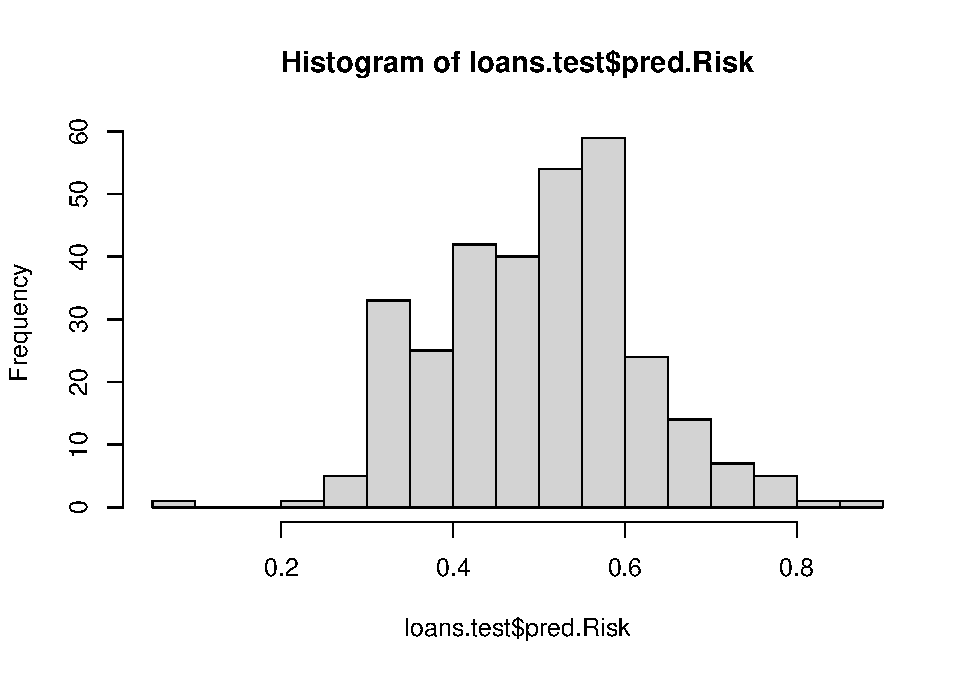
\includegraphics{classification1_files/figure-latex/unnamed-chunk-43-1.pdf}

Taking a look at the \texttt{pred.Risk} variable we appended to our
\texttt{loans.test} dataframe: we can therefore set a ``risk''
threshold, say, at 0.5 and predict any loans that exceed that threshold
as a ``default=1''. 0.5 may not always be the right threshold setting
and we'll discuss that later in the section describing ``precision'' vs
``recall''.

\begin{Shaded}
\begin{Highlighting}[]
\NormalTok{loans.test[}\DecValTok{1}\SpecialCharTok{:}\DecValTok{10}\NormalTok{, }\DecValTok{15}\SpecialCharTok{:}\DecValTok{17}\NormalTok{]}
\end{Highlighting}
\end{Shaded}

\begin{verbatim}
##    verified grdCtoA pred.Risk
## 6         0       1 0.3290653
## 8         0       1 0.4834721
## 9         1       0 0.5338793
## 10        1       0 0.5643251
## 26        1       0 0.6438010
## 38        1       0 0.6271196
## 39        1       0 0.5587168
## 41        0       1 0.3529768
## 42        1       1 0.3774766
## 44        1       0 0.7386618
\end{verbatim}

\hypertarget{exercise-prediction-output}{%
\subsubsection{Exercise: Prediction
Output}\label{exercise-prediction-output}}

As an exercise, try appending yet another variable (column) to the above
dataframe. Name it \texttt{pred.not\_paid} and make sure it's a binary
(0 or 1). You can use \texttt{ifelse} for this task.

If you succeed in the above task, compare using \texttt{table()} the
prediction you've made (\texttt{pred.not\_paid}) against the ``ground
truth'' which is in the \texttt{not\_paid} variable.

\begin{Shaded}
\begin{Highlighting}[]
\FunctionTok{table}\NormalTok{(}\StringTok{"predicted"}\OtherTok{=}\FunctionTok{as.numeric}\NormalTok{(loans.test}\SpecialCharTok{$}\NormalTok{pred.Risk}\SpecialCharTok{\textgreater{}=}\FloatTok{0.5}\NormalTok{), }\StringTok{"actual"}\OtherTok{=}\NormalTok{loans.test}\SpecialCharTok{$}\NormalTok{not\_paid)}
\end{Highlighting}
\end{Shaded}

\begin{verbatim}
##          actual
## predicted  0  1
##         0 93 54
##         1 68 97
\end{verbatim}

This table above is also known as the \textbf{confusion matrix}.

Observe from the confusion matrix that: - Out of the 151 actual defaults
we classified 97 of them correctly\\
- Out of the 161 fully-paid loans we classified 93 of them correctly\\
- Out of the 312 cases of loans in our test set, we classified 190 of
them correctly

\hypertarget{evaluating-classifiers-sensitivity-specificity-and-precision}{%
\subsection{Evaluating Classifiers: Sensitivity, Specificity and
Precision}\label{evaluating-classifiers-sensitivity-specificity-and-precision}}

Sensitivity and specificity are metrics commonly used to measures the
performance of a binary classification.

\begin{itemize}
\tightlist
\item
  Sensitivity (also called the true positive rate, the \textbf{recall},
  or probability of detection in some fields) measures the proportion of
  positives that are correctly identified as such (cancer cell
  detection, email spam, insurance fraud etc)\\
\item
  Specificity (also called the true negative rate) measures the
  proportion of negatives that are correctly identified as such
  (e.g.~the percentage of healthy people who are correctly identified as
  not having the condition, legitimate emails identified as such,
  legitimate insurance claims)\\
\item
  Precision: Proportion of correctly identified positives from all
  classified as such\\
\item
  Accuracy: Proportion of correctly identified cases from all cases
\end{itemize}

\begin{figure}
\centering
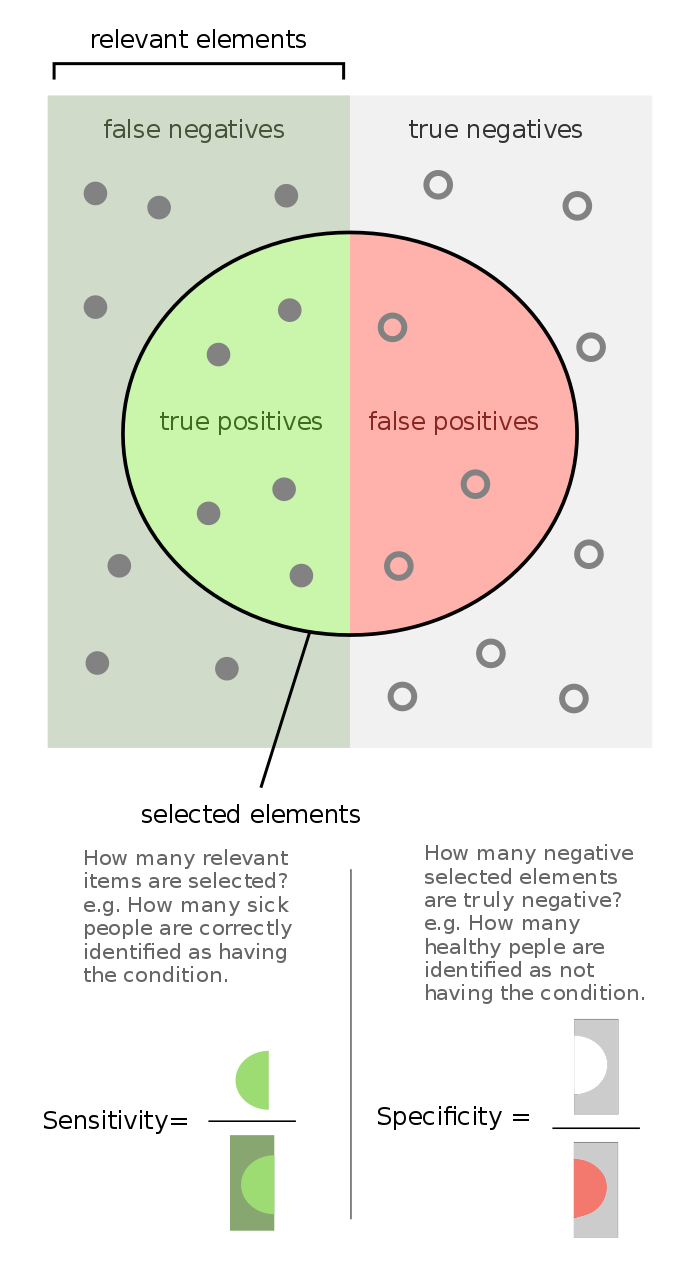
\includegraphics{assets/sensitivity.png}
\caption{Source: Wikipedia}
\end{figure}

Given the confusion matrix, can you describe the precision, recall, and
accuracy of our model?

\begin{Shaded}
\begin{Highlighting}[]
\FunctionTok{table}\NormalTok{(}\StringTok{"predicted"}\OtherTok{=}\FunctionTok{as.numeric}\NormalTok{(loans.test}\SpecialCharTok{$}\NormalTok{pred.Risk}\SpecialCharTok{\textgreater{}=}\FloatTok{0.5}\NormalTok{), }\StringTok{"actual"}\OtherTok{=}\NormalTok{loans.test}\SpecialCharTok{$}\NormalTok{not\_paid)}
\end{Highlighting}
\end{Shaded}

\begin{verbatim}
##          actual
## predicted  0  1
##         0 93 54
##         1 68 97
\end{verbatim}

\begin{Shaded}
\begin{Highlighting}[]
\NormalTok{accu }\OtherTok{\textless{}{-}} \FunctionTok{round}\NormalTok{((}\DecValTok{93}\SpecialCharTok{+}\DecValTok{97}\NormalTok{)}\SpecialCharTok{/}\FunctionTok{nrow}\NormalTok{(loans.test),}\DecValTok{2}\NormalTok{)}
\NormalTok{reca }\OtherTok{\textless{}{-}} \FunctionTok{round}\NormalTok{(}\DecValTok{97}\SpecialCharTok{/}\NormalTok{(}\DecValTok{54}\SpecialCharTok{+}\DecValTok{97}\NormalTok{),}\DecValTok{2}\NormalTok{)}
\NormalTok{prec }\OtherTok{\textless{}{-}} \FunctionTok{round}\NormalTok{(}\DecValTok{97}\SpecialCharTok{/}\NormalTok{(}\DecValTok{68}\SpecialCharTok{+}\DecValTok{97}\NormalTok{),}\DecValTok{2}\NormalTok{)}
\NormalTok{spec }\OtherTok{\textless{}{-}} \FunctionTok{round}\NormalTok{(}\DecValTok{93}\SpecialCharTok{/}\NormalTok{(}\DecValTok{93}\SpecialCharTok{+}\DecValTok{68}\NormalTok{),}\DecValTok{2}\NormalTok{)}

\FunctionTok{paste}\NormalTok{(}\StringTok{"Recall:"}\NormalTok{, reca)}
\end{Highlighting}
\end{Shaded}

\begin{verbatim}
## [1] "Recall: 0.64"
\end{verbatim}

\begin{Shaded}
\begin{Highlighting}[]
\FunctionTok{paste}\NormalTok{(}\StringTok{"Precision:"}\NormalTok{, prec)}
\end{Highlighting}
\end{Shaded}

\begin{verbatim}
## [1] "Precision: 0.59"
\end{verbatim}

\begin{Shaded}
\begin{Highlighting}[]
\FunctionTok{paste}\NormalTok{(}\StringTok{"Specificity:"}\NormalTok{, spec)}
\end{Highlighting}
\end{Shaded}

\begin{verbatim}
## [1] "Specificity: 0.58"
\end{verbatim}

\begin{Shaded}
\begin{Highlighting}[]
\FunctionTok{paste}\NormalTok{(}\StringTok{"Accuracy:"}\NormalTok{, accu)}
\end{Highlighting}
\end{Shaded}

\begin{verbatim}
## [1] "Accuracy: 0.61"
\end{verbatim}

Sometimes, you'll also find machine learning applications that uses the
notion of a baseline measure in their model evaluation phase. The
baseline performance is used to quantify the improvement of an applied
solution to the problem and a \textbf{base rate} is just the accuracy of
trivially predicting the most-frequent (or majority) class. An
implementation of this is the ZeroR Classifier found in many data mining
applications or related domains: since it ignores all predictors, ZeroR
ends us classifying according to the prior probability.

\begin{Shaded}
\begin{Highlighting}[]
\FunctionTok{prop.table}\NormalTok{(}\FunctionTok{table}\NormalTok{(loans.test}\SpecialCharTok{$}\NormalTok{not\_paid))}
\end{Highlighting}
\end{Shaded}

\begin{verbatim}
## 
##         0         1 
## 0.5160256 0.4839744
\end{verbatim}

Our baseline rate is 0.51 - a classifier that does no better than 0.51
is not useful because we might as well have classify every loan to the
majority class!

False negatives and false positives are rarely equally costly to a
business (or really, to any domain). For an insurance company, a false
negative on an insurance payout is likely to cost the company more than
a false positive for example. Finding the right precision-recall
tradeoff comes with domain expertise - and let's make all of these more
concrete by extending our credit risk example above.

Say the bank's credit department would rather sacrifice some level of
specificity or precision in favor of higher recall (or sensitivity). In
simpler words, we want to be more sensitive to ``loan defaults'', how
would you go about doing that? Try and think critically of the problem
before scrolling down to the proposed solution.

Well, one thing we can do is to set the threshold to be more sensitive
to ``positive cases'': Let's see what happen if we were to predict a
``default'' when the probability exceed 0.4 (20\% more sensitive than
our previous classifier):

\begin{Shaded}
\begin{Highlighting}[]
\FunctionTok{table}\NormalTok{(}\StringTok{"predicted"}\OtherTok{=}\FunctionTok{as.integer}\NormalTok{(loans.test}\SpecialCharTok{$}\NormalTok{pred.Risk}\SpecialCharTok{\textgreater{}=}\FloatTok{0.4}\NormalTok{), }\StringTok{"actual"}\OtherTok{=}\NormalTok{loans.test}\SpecialCharTok{$}\NormalTok{not\_paid)}
\end{Highlighting}
\end{Shaded}

\begin{verbatim}
##          actual
## predicted   0   1
##         0  43  22
##         1 118 129
\end{verbatim}

We increased our Sensitivity or Recall rate from 0.64 to above 0.85!
What is the cost of such an adjustment?

\hypertarget{performance-evaluation-and-model-selection}{%
\subsubsection{Performance evaluation and model
selection}\label{performance-evaluation-and-model-selection}}

On top of what we've learned so far, there are other tools we can use to
evaluate and compare between the performances of our regression models:

\textbf{1. AIC (Akaike Information Criteria)}\\
Like R-squared, AIC is a statistical measure of how close the data are
to the fitted regression line. It gives us a measure of fit: we'll
therefore choose the model with the lowest AIC value, as it helps us
minimize residual error in our model:

\begin{Shaded}
\begin{Highlighting}[]
\NormalTok{honors.aic }\OtherTok{\textless{}{-}} \FunctionTok{paste}\NormalTok{(honors.logit}\SpecialCharTok{$}\NormalTok{aic, }\StringTok{"}\SpecialCharTok{\textbackslash{}n}\StringTok{"}\NormalTok{, honors.logit2}\SpecialCharTok{$}\NormalTok{aic, }\StringTok{"}\SpecialCharTok{\textbackslash{}n}\StringTok{"}\NormalTok{, honors.logit3}\SpecialCharTok{$}\NormalTok{aic, }\StringTok{"}\SpecialCharTok{\textbackslash{}n}\StringTok{"}\NormalTok{, honors.logit4}\SpecialCharTok{$}\NormalTok{aic)}

\FunctionTok{cat}\NormalTok{(honors.aic)}
\end{Highlighting}
\end{Shaded}

\begin{verbatim}
## 224.710046686266 
##  223.606248275242 
##  171.073237223271 
##  164.169552365161
\end{verbatim}

However, unlike adjusted R-squared, the number itself is not meaningful.
If you have more than one similar candidate models (where all of the
variables of the simpler model occur in the more complex models), then
you should select the model that has the smallest AIC.

\begin{Shaded}
\begin{Highlighting}[]
\FunctionTok{AIC}\NormalTok{(honors.logit4)}
\end{Highlighting}
\end{Shaded}

\begin{verbatim}
## [1] 164.1696
\end{verbatim}

\textbf{2. Null Deviance and Residual Deviance} Null deviance indicates
how well the response variable is predicted by a model that includes
only the intercept (grand mean). The residual deviance shows how well
the response variable is predicted by the model when all predictors are
included.

Intuitively, this means our first model - with no predictor variables
\texttt{glm(hon\ \textasciitilde{}\ 1)} should see the same null
deviance and residual deviance, and it is (table below)!

As we add more / subtract predictor variables, notice how our residual
deviance change.

\begin{Shaded}
\begin{Highlighting}[]
\NormalTok{honors.null.resi }\OtherTok{\textless{}{-}} \FunctionTok{paste}\NormalTok{(honors.logit}\SpecialCharTok{$}\NormalTok{null.deviance, }\StringTok{"\textbackslash{} "}\NormalTok{, honors.logit}\SpecialCharTok{$}\NormalTok{deviance, }\StringTok{"}\SpecialCharTok{\textbackslash{}n}\StringTok{"}\NormalTok{, honors.logit2}\SpecialCharTok{$}\NormalTok{null.deviance, }\StringTok{"\textbackslash{} "}\NormalTok{, honors.logit2}\SpecialCharTok{$}\NormalTok{deviance, }\StringTok{"}\SpecialCharTok{\textbackslash{}n}\StringTok{"}\NormalTok{, honors.logit3}\SpecialCharTok{$}\NormalTok{null.deviance, }\StringTok{"\textbackslash{} "}\NormalTok{, honors.logit3}\SpecialCharTok{$}\NormalTok{deviance, }\StringTok{"}\SpecialCharTok{\textbackslash{}n}\StringTok{"}\NormalTok{, honors.logit4}\SpecialCharTok{$}\NormalTok{null.deviance, }\StringTok{"\textbackslash{} "}\NormalTok{, honors.logit4}\SpecialCharTok{$}\NormalTok{deviance, }\StringTok{"}\SpecialCharTok{\textbackslash{}n}\StringTok{"}\NormalTok{)}

\FunctionTok{cat}\NormalTok{(honors.null.resi)}
\end{Highlighting}
\end{Shaded}

\begin{verbatim}
## 222.710046686266   222.710046686266 
##  222.710046686266   219.606248275242 
##  222.710046686266   167.073237223271 
##  222.710046686266   156.169552365161
\end{verbatim}

\begin{Shaded}
\begin{Highlighting}[]
\NormalTok{honors.train }\OtherTok{\textless{}{-}}\NormalTok{ honors[}\DecValTok{1}\SpecialCharTok{:}\DecValTok{150}\NormalTok{,]}
\NormalTok{honors.test }\OtherTok{\textless{}{-}}\NormalTok{ honors[}\DecValTok{151}\SpecialCharTok{:}\DecValTok{200}\NormalTok{,]}
\NormalTok{honors.logit5 }\OtherTok{\textless{}{-}} \FunctionTok{glm}\NormalTok{(hon }\SpecialCharTok{\textasciitilde{}}\NormalTok{ female }\SpecialCharTok{+}\NormalTok{ read }\SpecialCharTok{+}\NormalTok{ math }\SpecialCharTok{+}\NormalTok{ write, }\AttributeTok{data=}\NormalTok{honors.train, }\AttributeTok{family=}\StringTok{"binomial"}\NormalTok{)}
\end{Highlighting}
\end{Shaded}

\begin{verbatim}
## Warning: glm.fit: algorithm did not converge
\end{verbatim}

\begin{verbatim}
## Warning: glm.fit: fitted probabilities numerically 0 or 1 occurred
\end{verbatim}

\begin{Shaded}
\begin{Highlighting}[]
\FunctionTok{summary}\NormalTok{(honors.logit5)}
\end{Highlighting}
\end{Shaded}

\begin{verbatim}
## 
## Call:
## glm(formula = hon ~ female + read + math + write, family = "binomial", 
##     data = honors.train)
## 
## Deviance Residuals: 
##          Min            1Q        Median            3Q           Max  
## -0.000143837  -0.000000021  -0.000000021  -0.000000021   0.000137952  
## 
## Coefficients:
##                 Estimate   Std. Error z value Pr(>|z|)
## (Intercept)  -1687.32338 290654.07075  -0.006    0.995
## female          -5.74849  11781.56200   0.000    1.000
## read             0.05895    703.91719   0.000    1.000
## math            -1.08072    527.47367  -0.002    0.998
## write           28.99738   5028.05044   0.006    0.995
## 
## (Dispersion parameter for binomial family taken to be 1)
## 
##     Null deviance: 155.501919075797  on 149  degrees of freedom
## Residual deviance:   0.000000071258  on 145  degrees of freedom
## AIC: 10
## 
## Number of Fisher Scoring iterations: 25
\end{verbatim}

Notice in the last model \texttt{honors.logit5}, we obtain an
unrealistically small residual deviance and coefficients that are
confusingly large. This is indicative of the ``Hauck Donner effect'':
This is when the fitted probabilities are extremely close to zero or
one. Consider a medical diagnosis problem with thousands of cases and
around 50 binary explanatory variable (which may arise from coding fewer
categorical variables); one of these indicators is rarely true but
always indicates that the disease is present. Then the fitted
probabilities of cases with that indicator should be one, which can only
be achieved by taking \(\beta_i\) = Inf. The result from glm will be
warnings and an estimated coefficient of around +/- 10\footnote{\href{https://books.google.co.id/books?hl=en\&lr=\&id=tovgBwAAQBAJ\&oi=fnd\&pg=PR11\&ots=eWKoGdCjkH\&sig=DGYBL1Mu-JW5qf8xhbfNZxetYLA\&redir_esc=y\#v=onepage\&q\&f=false}{Modern
  Applied Statistics with S-Plus}}.

\begin{Shaded}
\begin{Highlighting}[]
\FunctionTok{exp}\NormalTok{(}\FunctionTok{coef}\NormalTok{(honors.logit5)[}\DecValTok{5}\NormalTok{])}
\end{Highlighting}
\end{Shaded}

\begin{verbatim}
##         write 
## 3921051194980
\end{verbatim}

\begin{Shaded}
\begin{Highlighting}[]
\CommentTok{\# Infinity minus any arbitarily large numbers still exceed 0.5}
\ConstantTok{Inf}\DecValTok{{-}1000000} \SpecialCharTok{\textgreater{}} \FloatTok{0.5}
\end{Highlighting}
\end{Shaded}

\begin{verbatim}
## [1] TRUE
\end{verbatim}

More intuition: This phenomenon where one or more predictors take on a
coefficient value of infinity is sometimes referred to as \emph{perfect
separation}. Another example: imagine the scenario where reading
\textgreater= 43 will perfectly predict honors=TRUE and reading
\textless{} 43 will perfectly predict honors=FALSE, or where
stock\_opening \textgreater= +3.34\% will perfectly predict end\_high =
TRUE and vice versa, then we can imagine that the probabilities where
such cases do happen must be 1, and that is achieved by setting the
coefficient to infinity.

\hypertarget{nearest-neighbor-algorithm}{%
\section{Nearest Neighbor Algorithm}\label{nearest-neighbor-algorithm}}

The k-nearest neighbor algorithm gets it name from the fact that it uses
information about an example's k-nearest neighbors to classify unlabeled
examples. Upon choosing \emph{k}, the algorithm requires a training
dataset made up of examples that have been classified into several
categories, as labeled by a nominal variable. Then, for each unlabeled
record in the test dataset, k-NN identifies \emph{k} records in the
training data that are the ``nearest'' in similarity. The unlabeled test
instance is assigned the class of the majority of the k-nearest
neighbors.

Supposed we pick k=1, then the * in the following feature space will be
assigned the square class, but if k=5, then the majority class of the
five nearest point will be assigned to that point and our point will be
classified as a round instead. 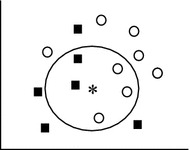
\includegraphics{assets/knn.jpg}

\hypertarget{motivational-example-is-tomato-a-fruit}{%
\subsection{Motivational Example: Is Tomato a
fruit?}\label{motivational-example-is-tomato-a-fruit}}

Suppose that prior to a blind tasting (or blind dining) experience, we
created a dataset in which we recorded our impressions of a number of
ingredients. For each ingredient, we rated its \texttt{sweetness} and
\texttt{crunchiness} and then labeled them as one of the three types of
food: \emph{fruits}, \emph{vegetables}, or \emph{proteins}.

\begin{Shaded}
\begin{Highlighting}[]
\CommentTok{\# Create our dataset}
\NormalTok{food }\OtherTok{\textless{}{-}} \FunctionTok{data.frame}\NormalTok{(}\FunctionTok{list}\NormalTok{(}\FunctionTok{c}\NormalTok{(}\StringTok{"apple"}\NormalTok{, }\StringTok{"bacon"}\NormalTok{, }\StringTok{"banana"}\NormalTok{, }\StringTok{"carrot"}\NormalTok{,}\StringTok{"celery"}\NormalTok{, }\StringTok{"cheese"}\NormalTok{,}\StringTok{"cucumber"}\NormalTok{, }\StringTok{"fish"}\NormalTok{, }\StringTok{"grape"}\NormalTok{, }\StringTok{"green bean"}\NormalTok{, }\StringTok{"lettuce"}\NormalTok{, }\StringTok{"nuts"}\NormalTok{, }\StringTok{"pear"}\NormalTok{, }\StringTok{"shrimp"}\NormalTok{,}\StringTok{"orange"}\NormalTok{), }\FunctionTok{c}\NormalTok{(}\DecValTok{10}\NormalTok{,}\DecValTok{1}\NormalTok{,}\DecValTok{10}\NormalTok{,}\DecValTok{6}\NormalTok{,}\DecValTok{3}\NormalTok{,}\DecValTok{1}\NormalTok{,}\DecValTok{2}\NormalTok{,}\DecValTok{3}\NormalTok{,}\DecValTok{10}\NormalTok{,}\DecValTok{3}\NormalTok{,}\DecValTok{1}\NormalTok{,}\DecValTok{3}\NormalTok{,}\DecValTok{10}\NormalTok{,}\DecValTok{2}\NormalTok{,}\DecValTok{9}\NormalTok{), }\FunctionTok{c}\NormalTok{(}\DecValTok{9}\NormalTok{,}\DecValTok{4}\NormalTok{,}\DecValTok{1}\NormalTok{,}\DecValTok{10}\NormalTok{,}\DecValTok{10}\NormalTok{,}\DecValTok{1}\NormalTok{,}\DecValTok{8}\NormalTok{,}\DecValTok{2}\NormalTok{,}\DecValTok{5}\NormalTok{,}\DecValTok{7}\NormalTok{,}\DecValTok{10}\NormalTok{,}\DecValTok{5}\NormalTok{,}\DecValTok{7}\NormalTok{,}\DecValTok{2}\NormalTok{,}\DecValTok{3}\NormalTok{), }\FunctionTok{c}\NormalTok{(}\StringTok{"fruit"}\NormalTok{, }\StringTok{"protein"}\NormalTok{, }\StringTok{"fruit"}\NormalTok{, }\StringTok{"vegetable"}\NormalTok{, }\StringTok{"vegetable"}\NormalTok{, }\StringTok{"protein"}\NormalTok{, }\StringTok{"vegetable"}\NormalTok{, }\StringTok{"protein"}\NormalTok{, }\StringTok{"fruit"}\NormalTok{, }\StringTok{"vegetable"}\NormalTok{, }\StringTok{"vegetable"}\NormalTok{, }\StringTok{"proteins"}\NormalTok{, }\StringTok{"fruit"}\NormalTok{,}\StringTok{"protein"}\NormalTok{, }\StringTok{"fruit"}\NormalTok{)))}

\CommentTok{\# Give each feature appropriate names}
\FunctionTok{colnames}\NormalTok{(food)}\OtherTok{\textless{}{-}} \FunctionTok{c}\NormalTok{(}\StringTok{"Ingredient"}\NormalTok{, }\StringTok{"Sweetness"}\NormalTok{, }\StringTok{"Crunchiness"}\NormalTok{, }\StringTok{"Type"}\NormalTok{)}
\end{Highlighting}
\end{Shaded}

The k-NN algorithm treats the features as coordinates in a
multidimensional feature space. As our dataset includes only two
features, the feature space is two-dimensional. We can plot
two-dimensional data on a scatterplot:

\begin{Shaded}
\begin{Highlighting}[]
\FunctionTok{library}\NormalTok{(ggplot2)}

\NormalTok{plot.fruit }\OtherTok{\textless{}{-}} \FunctionTok{ggplot}\NormalTok{(food, }\FunctionTok{aes}\NormalTok{(}\AttributeTok{x=}\NormalTok{Sweetness, }\AttributeTok{y=}\NormalTok{Crunchiness)) }\SpecialCharTok{+} 
  \FunctionTok{geom\_point}\NormalTok{(}\AttributeTok{alpha =} \FloatTok{0.05}\NormalTok{)}\SpecialCharTok{+}\FunctionTok{geom\_label}\NormalTok{(}\FunctionTok{aes}\NormalTok{(}\AttributeTok{label=}\NormalTok{Ingredient),}
                                      \AttributeTok{nudge\_x=}\FloatTok{0.5}\NormalTok{, }\AttributeTok{nudge\_y=}\DecValTok{0}\NormalTok{, }\AttributeTok{label.size=}\FloatTok{0.6}\NormalTok{) }\SpecialCharTok{+} 
  \FunctionTok{labs}\NormalTok{(}\AttributeTok{x=}\StringTok{"how sweet the food tastes"}\NormalTok{, }\AttributeTok{y=}\StringTok{"how crunchy the food is"}\NormalTok{)}
\NormalTok{plot.fruit}
\end{Highlighting}
\end{Shaded}

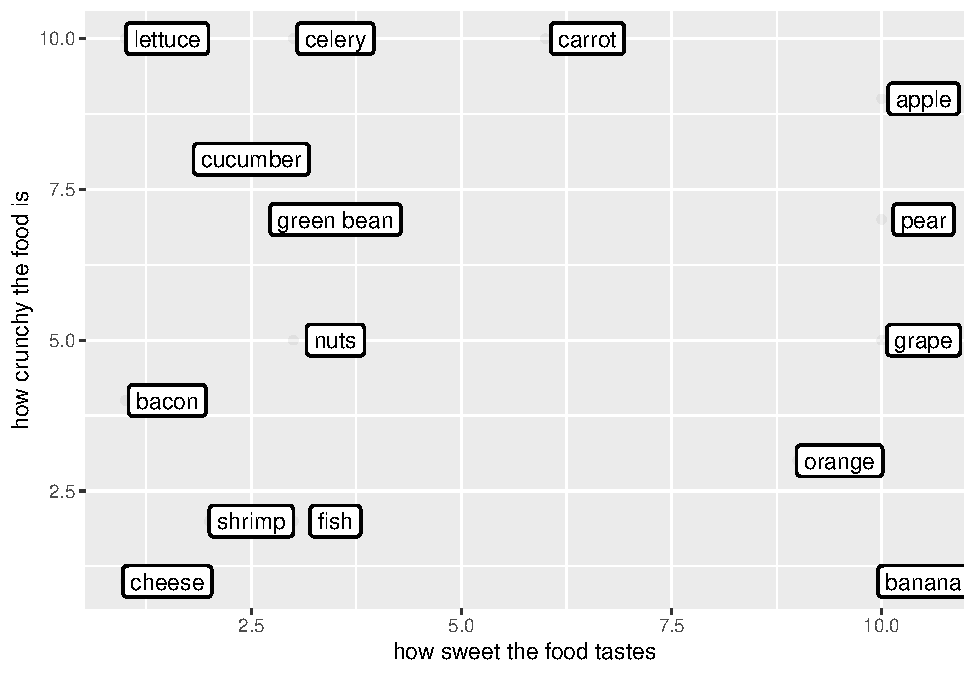
\includegraphics{classification1_files/figure-latex/unnamed-chunk-56-1.pdf}
Observe here that similar types of food tend to be grouped closely
together.

Supposed we'd like to decide if tomato is a fruit or a vegetable, we
would put tomato onto our dataset:

\begin{Shaded}
\begin{Highlighting}[]
\FunctionTok{library}\NormalTok{(grid)}
\NormalTok{grob }\OtherTok{=} \FunctionTok{grobTree}\NormalTok{(}\FunctionTok{textGrob}\NormalTok{(}\StringTok{"tomato"}\NormalTok{, }\AttributeTok{x=}\FloatTok{0.6}\NormalTok{, }\AttributeTok{y=}\FloatTok{0.4}\NormalTok{, }\AttributeTok{hjust=}\DecValTok{0}\NormalTok{, }\AttributeTok{gp=}\FunctionTok{gpar}\NormalTok{(}\AttributeTok{col=}\StringTok{"darkorange"}\NormalTok{, }\AttributeTok{fontsize=}\DecValTok{14}\NormalTok{)))}

\NormalTok{plot.fruit }\SpecialCharTok{+} \FunctionTok{annotation\_custom}\NormalTok{(grob)}
\end{Highlighting}
\end{Shaded}

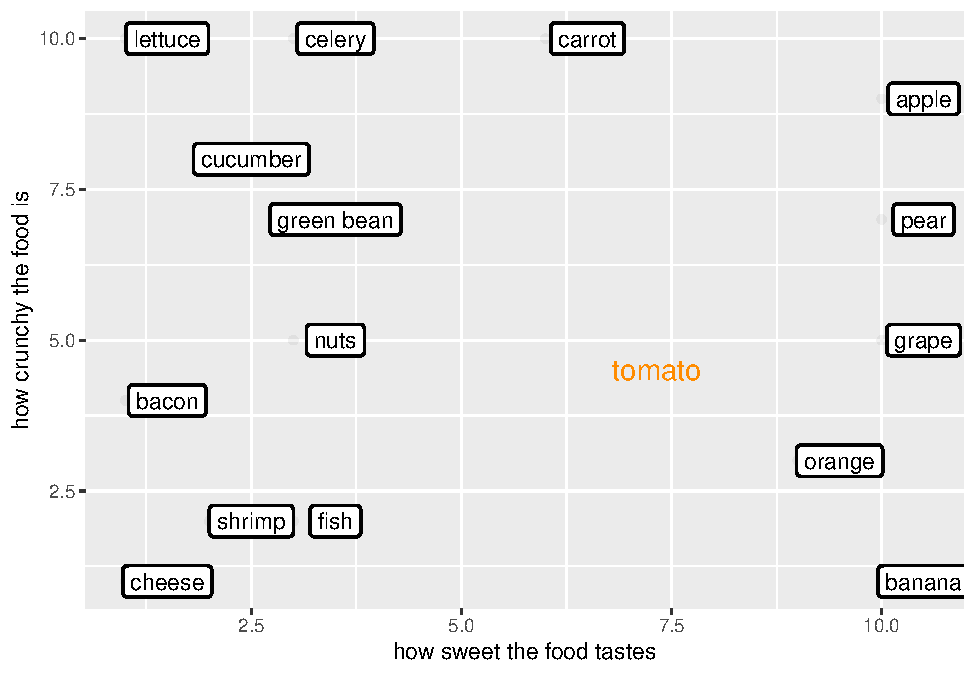
\includegraphics{classification1_files/figure-latex/unnamed-chunk-57-1.pdf}

With that we would then use a \emph{distance function} to find tomato's
nearest neighbors. Traditionally, the k-NN algorithm assumes
\emph{Euclidean distance}, which is the shortest direct route (imagine
using a ruler to connect two points). While Euclidean distance function
is the most widely used distance metric in k-NN, you will sometimes see
the Manhattan distance (which is based on the paths a pedestrian would
take by walking city blocks) being used instead \footnote{\href{https://www.ncbi.nlm.nih.gov/pmc/articles/PMC4978658/}{Hu
  LY, et. al (2016), The distance function effect on k-nearest neighbor
  classification for medical datasets}}.

A few academic papers on this literature may also reference the
Minkowsky distance function\footnote{Batchelor BG. Pattern recognition:
  ideas in practice. Berlin, Heidelberg: Plenum Press; 1978.}:\\
dist\_Minkowsky(A,B) =
\((\sum\limits^m_{i=1} |x_i -y_i|^r)^{\frac{1}{r}}\)

While these distance functions exist, Euclidean distance is far more
often seen in industrial applications and is therefore the focus of this
chapter. As a side note, Minkowsky distance is typically used with
\emph{r} being 1 or 2, where the former is equivalent to the Manhattan
distance while the latter is the Euclidean distance.

\hypertarget{euclidean-distance}{%
\subsubsection{Euclidean Distance}\label{euclidean-distance}}

Let A and B be represented by feature vectors A = (\(x_1, x_2, …, x_m\))
and B = (\(y_1, y_2, …, y_m\)), where \emph{m} is the dimensionality of
the feature space. To calculate the distance between A and B, the
Euclidean Distance formula can be represented as such:

dist(A, B) = \(\sqrt{\sum\limits^{m}_{i=1}(x_i-y_i)^2}\)

Applying the above formula on our blind-tasting example, we can
calculate the distance between:\\
- tomato (sweet: 6, crunchy: 4)\\
- green bean (sweet: 3, crunchy: 7)

dist(tomato, greenbean) = \texttt{sqrt((6-3)\^{}2\ +\ (4-7)\^{}2))},
which is 4.24

Similarly, we can calculate the distance between the tomato and several
of its closest neighbors. Supposed we've done that and choose to assign
tomato the food type of its nearest neighbor, which in our case is the
orange (distance: 1.4), we are doing what is formally a 1-NN
classification. Under 1-NN then the orange would be classified as a
fruit.

Had we use the k-NN with 3 nearest neighbor instead: orange, grape, and
nuts, the majority vote (2 fruits vs 1 protein) would again classify the
tomato as a fruit.

\hypertarget{choosing-an-appropriate-k}{%
\subsubsection{\texorpdfstring{Choosing an appropriate
\emph{k}}{Choosing an appropriate k}}\label{choosing-an-appropriate-k}}

The decision of how many neighbors to use for k-NN determines how well
the model will generalize to future data. The balance between
overfitting and underfitting the training data is a problem known as
\textbf{bias-variance tradeoff}. Choosing a large k reduces the impact
or variance caused by noisy data, but can bias the learner so that it
runs the risk of ignoring small, but important patterns.

If we use a very large \emph{k}, say, a \emph{k} value as large as the
total number of observations in the training data, this would lead to
the always predicting the majority class (ZeroR classifier), which we've
learned about in the previous chapter.

On the opposite extreme, using a single nearest neighbor allows the
noisy data or outliers to unduly influence the classification of
examples. If one of our training examples were accidentally mislabeled
and happens to be a neighboring data point, choosing a k=1 will have
resulted in a misclassification, even if the nine other nearest
neighbors would have voted differently.

In practice, one common strategy is to begin with \emph{k} equal to the
square root of the number of training examples. Another strategy is to
choose a larger k but apply a weighted voting process in which the vote
of the closer neighbors is considered more authoritative than the vote
of the farther away neighbors.

\hypertarget{features-rescaling}{%
\subsubsection{Features rescaling}\label{features-rescaling}}

Supposed, in addition to Sweetness and Crunchiness, we add a new feature
``Spiciness'' which is measured on a scale of 0 to 10,000. This range,
or difference in scale, will allow the spice level of a food to have an
amplified impact on the distance function. In fact, it's enlarged
contribution to the distance function may end up being the singular
decisive feature!

We solve this by rescaling the features, i.e shrinking or expanding
their range so that each feature's contribution to the distance formula
is equally weighed. We want spiciness to be measured on the same scale
as sweetness and crunchiness, which is a scale from 1 to 10. The two
methods of rescaling features are:

\begin{itemize}
\tightlist
\item
  Mix-Max normalization\\
\item
  z-score standardization
\end{itemize}

\textbf{Min-max normalization} works by transforming a feature such that
its values fall into a range of 0 to 1.

The formula: \(x_{new}\) = \texttt{(x-min(x))\ /\ (max(x)\ -\ min(x))}

\begin{itemize}
\tightlist
\item
  Which essentially subtracts the min of feature \emph{x} from each
  value and divides by the range of \emph{x}.
\end{itemize}

Normalized feature's values effectively communicates how far, in
percentage terms, the original value fell along the range of all values
of feature \emph{x}.

\textbf{z-score standardization} on the other hand subtracts the mean
value of feature \emph{x} and divides the outcome by the standard
deviation of \emph{x}.

The formula: \(x_{new}\) = \texttt{(x-mean(x))/sd(x)}

Standardization rescales each of the feature's values in terms of how
many standard deviations they fall above or below the mean values. The
resulting value is called a \emph{z-score}. Z-scores has no predefined
bounds (minimum and maximum) and may be negative or positive numbers. A
more detailed discussion of this is in the Practical Statistics
coursebook you have received in an earlier workshop.

\hypertarget{characteristics-of-k-nn}{%
\subsubsection{Characteristics of k-NN}\label{characteristics-of-k-nn}}

Classification methods using k-NN are called `lazy learners'. Lazy
learners do not build a model; There is no abstraction or generalization
process -- compare this to the logistic regression method we've learned
earlier to have an intuition of what `building a model' means. More
technically, we say that no `parameters' are learned about the data.

Let's summarize the process that goes into prediction with a k-NN
classifier:\\
- Scaling (putting the variables on a same scale to avoid one variable
overpowering the others)\\
- Select a positive integer \emph{k}\\
- Select the \emph{k} nearest neighbor for each ``test'' sample\\
- Classify based on majority class

Because k-NN makes prediction in a manner that is ``just-in-time'' by
calculating the similarity between each input sample and the other
training samples in the vector space, this method may be computationally
expensive on dataset with high dimensionality (high memory requirement
and constantly calculating ``distances'' over and over again). If we
pick a small \emph{k} value, our algorithm may also be vulnerable to the
``noise'' in our data. On its own, it is also sensitive to the ``scale''
of our data.

Despite the limitations, k-NN is incredibly powerful and versatile. In
fact some of its weaknesses (such as the outlier and scales) can be
adequately mitigated with the scaling strategy we've learned in the
earlier section. It is also generally insensitive to outlier and noise
when an appropriate \emph{k} value is picked. Unlike logistic regression
or linear regression, it works well on non-linear data because k-NN does
not make assumption about the data.

Under specific settings and requirements, k-NN is some of the most
extensively used algorithms and have impressive accuracy. However, its
performance is not competitive compared to ensemble methods (a key focus
of our next workshop, ``Classification 2'') and has even seen its fair
share of application in regression problems!

An example of Nearest Neighbor being used in performance benchmarking by
the Microsoft's Kinect team: 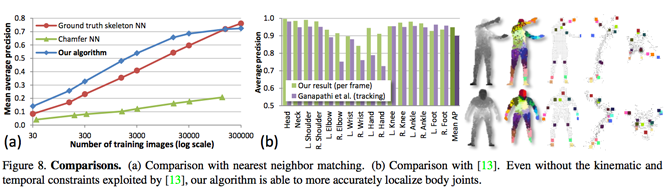
\includegraphics{assets/kinect.png} Read:
\url{http://research.microsoft.com/pubs/145347/BodyPartRecognition.pdf}

\hypertarget{diagnosing-breast-cancer-with-the-k-nn-algorithm}{%
\subsection{Diagnosing breast cancer with the k-NN
algorithm}\label{diagnosing-breast-cancer-with-the-k-nn-algorithm}}

For this example, we use the Winconsin Breast Cancer Diagnostic dataset
from the UCI Machine Learning repository
\href{http://pubsonline.informs.org/doi/abs/10.1287/opre.43.4.570?journalCode=opre}{read
more}. This dataset includes 569 examples of cancer biopsies, each with
32 features. One feature is an identification number, another is the
cancer diagnosis, and 30 are numeric-valued laboratory measurements. The
diagnosis is coded as ``M'' to indicate malignant or ``B'' to indicate
benign.

The 30 numeric measurements includes the mean, standard error, and worst
value for 10 different characteristics of the digitalized cell nuclei
(radius, texture, symmetry, area etc)

\begin{Shaded}
\begin{Highlighting}[]
\CommentTok{\# importing the data and quickly explore the first 5 variables of the dataset}
\NormalTok{wbcd }\OtherTok{\textless{}{-}} \FunctionTok{read.csv}\NormalTok{(}\StringTok{"data\_input/wisc\_bc\_data.csv"}\NormalTok{)}
\FunctionTok{str}\NormalTok{(wbcd[,}\DecValTok{1}\SpecialCharTok{:}\DecValTok{5}\NormalTok{])}
\end{Highlighting}
\end{Shaded}

\begin{verbatim}
## 'data.frame':    569 obs. of  5 variables:
##  $ id            : int  87139402 8910251 905520 868871 9012568 906539 925291 87880 862989 89827 ...
##  $ diagnosis     : chr  "B" "B" "B" "B" ...
##  $ radius_mean   : num  12.3 10.6 11 11.3 15.2 ...
##  $ texture_mean  : num  12.4 18.9 16.8 13.4 13.2 ...
##  $ perimeter_mean: num  78.8 69.3 70.9 73 97.7 ...
\end{verbatim}

Seeing that the \texttt{id} variable provides no valuable information
(or worse, it may lead to ``noise'' in our learning task later) we
should eliminate this feature

\begin{Shaded}
\begin{Highlighting}[]
\NormalTok{wbcd }\OtherTok{\textless{}{-}}\NormalTok{ wbcd[,}\SpecialCharTok{{-}}\DecValTok{1}\NormalTok{]}
\end{Highlighting}
\end{Shaded}

The \texttt{diagnosis} variable is of special interest to us, because it
is the \textbf{target feature}, or simply put, it is the outcome we like
to predict. It's a \texttt{character} class vector - let's convert it to
a factor as well as a more descriptive label

\begin{Shaded}
\begin{Highlighting}[]
\NormalTok{wbcd}\SpecialCharTok{$}\NormalTok{diagnosis }\OtherTok{\textless{}{-}} \FunctionTok{factor}\NormalTok{(wbcd}\SpecialCharTok{$}\NormalTok{diagnosis, }\AttributeTok{levels =} \FunctionTok{c}\NormalTok{(}\StringTok{"B"}\NormalTok{, }\StringTok{"M"}\NormalTok{), }\AttributeTok{labels =} \FunctionTok{c}\NormalTok{(}\StringTok{"Benign"}\NormalTok{, }\StringTok{"Malignant"}\NormalTok{))}
\FunctionTok{table}\NormalTok{(wbcd}\SpecialCharTok{$}\NormalTok{diagnosis)}
\end{Highlighting}
\end{Shaded}

\begin{verbatim}
## 
##    Benign Malignant 
##       357       212
\end{verbatim}

We could as easily see the proportion table by wrapping the call to
\texttt{table()} in a \texttt{prop.table} function:

\begin{Shaded}
\begin{Highlighting}[]
\FunctionTok{round}\NormalTok{(}\FunctionTok{prop.table}\NormalTok{(}\FunctionTok{table}\NormalTok{(wbcd}\SpecialCharTok{$}\NormalTok{diagnosis))}\SpecialCharTok{*}\DecValTok{100}\NormalTok{,}\DecValTok{1}\NormalTok{)}
\end{Highlighting}
\end{Shaded}

\begin{verbatim}
## 
##    Benign Malignant 
##      62.7      37.3
\end{verbatim}

The remaining 30 features are all numeric, and we can further
investigate their relationship with each other using a matrix of
scatterplots

\begin{Shaded}
\begin{Highlighting}[]
\CommentTok{\# Find any patterns of relationship between our 2nd and 6th features}
\FunctionTok{pairs}\NormalTok{(wbcd[,}\DecValTok{2}\SpecialCharTok{:}\DecValTok{6}\NormalTok{])}
\end{Highlighting}
\end{Shaded}

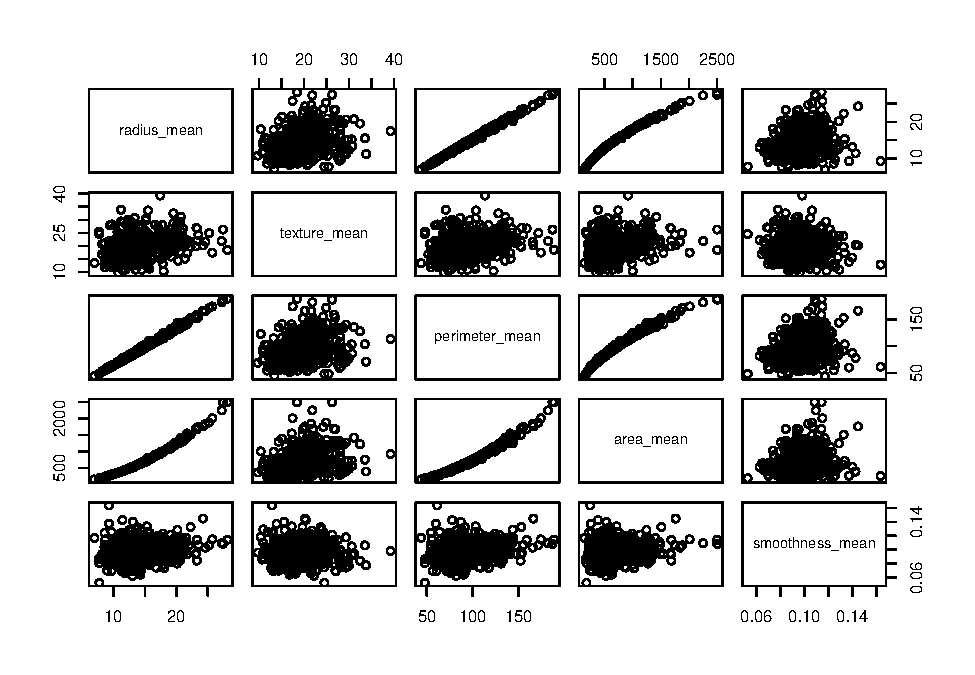
\includegraphics{classification1_files/figure-latex/unnamed-chunk-62-1.pdf}

Not surprisingly, we see that \texttt{radius}, \texttt{perimeter} and
\texttt{area} are strongly related, in an almost linear fashion.
Recalling from our geometry classes, this makes a lot of sense! Of
course, a numerical version of the scatterplots above would be
\texttt{cor}:

\begin{Shaded}
\begin{Highlighting}[]
\FunctionTok{cor}\NormalTok{(wbcd[,}\DecValTok{2}\SpecialCharTok{:}\DecValTok{6}\NormalTok{])}
\end{Highlighting}
\end{Shaded}

\begin{verbatim}
##                 radius_mean texture_mean perimeter_mean area_mean
## radius_mean       1.0000000   0.32378189      0.9978553 0.9873572
## texture_mean      0.3237819   1.00000000      0.3295331 0.3210857
## perimeter_mean    0.9978553   0.32953306      1.0000000 0.9865068
## area_mean         0.9873572   0.32108570      0.9865068 1.0000000
## smoothness_mean   0.1705812  -0.02338852      0.2072782 0.1770284
##                 smoothness_mean
## radius_mean          0.17058119
## texture_mean        -0.02338852
## perimeter_mean       0.20727816
## area_mean            0.17702838
## smoothness_mean      1.00000000
\end{verbatim}

If we're paying attention, we also notice that the features have varying
measurement scales! Radius, area, compactness and symmetry for example
have a different range of values and will require normalization.

Let's create our normalize function:

\begin{Shaded}
\begin{Highlighting}[]
\CommentTok{\# Creating a normalize() function, which takes a vector x and for each value in that vector, subtracts the minimum value in x and divides by the range of x}

\NormalTok{normalize }\OtherTok{\textless{}{-}} \ControlFlowTok{function}\NormalTok{(x)\{}
  \FunctionTok{return}\NormalTok{ ( }
\NormalTok{    (x }\SpecialCharTok{{-}} \FunctionTok{min}\NormalTok{(x))}\SpecialCharTok{/}\NormalTok{(}\FunctionTok{max}\NormalTok{(x) }\SpecialCharTok{{-}} \FunctionTok{min}\NormalTok{(x)) }
\NormalTok{  )}
\NormalTok{\}}
\end{Highlighting}
\end{Shaded}

Notice we could also have use \texttt{diff(range(x))} instead of
\texttt{max(x)\ -\ min(x)}. \texttt{range(x)} returns a vector of two,
the min and max, so diff() will calculate the difference between that
two value. Let's test our normalize functions on a few vectors:

\begin{Shaded}
\begin{Highlighting}[]
\FunctionTok{normalize}\NormalTok{(}\FunctionTok{c}\NormalTok{(}\DecValTok{1}\NormalTok{,}\DecValTok{2}\NormalTok{,}\DecValTok{3}\NormalTok{,}\DecValTok{4}\NormalTok{,}\DecValTok{5}\NormalTok{))}
\end{Highlighting}
\end{Shaded}

\begin{verbatim}
## [1] 0.00 0.25 0.50 0.75 1.00
\end{verbatim}

\begin{Shaded}
\begin{Highlighting}[]
\FunctionTok{normalize}\NormalTok{(}\FunctionTok{c}\NormalTok{(}\DecValTok{2000}\NormalTok{, }\DecValTok{2500}\NormalTok{, }\DecValTok{3000}\NormalTok{, }\DecValTok{2800}\NormalTok{))}
\end{Highlighting}
\end{Shaded}

\begin{verbatim}
## [1] 0.0 0.5 1.0 0.8
\end{verbatim}

We observe that despite the second vector being a lot larger, they are
normalized into the same range (0 to 1). We can now safely apply this
function using \texttt{lapply}. \texttt{lapply} applies a specified
function to each list element -- and a data frame is just a list of
equal-length vectors. \texttt{lapply} returns a list, so we'll use
\texttt{as.data.frame} to convert it back to a data frame:

\begin{Shaded}
\begin{Highlighting}[]
\CommentTok{\# we also drop the diagnosis outcome variable in the new dataframe, hence [2:31]}
\NormalTok{wbcd\_n }\OtherTok{\textless{}{-}} \FunctionTok{data.frame}\NormalTok{(}\FunctionTok{lapply}\NormalTok{(wbcd[,}\DecValTok{2}\SpecialCharTok{:}\DecValTok{31}\NormalTok{], normalize))}
\end{Highlighting}
\end{Shaded}

Where before we have values from 0 all up to thousands, we now have
values of 0 to 1 for all features

\begin{Shaded}
\begin{Highlighting}[]
\FunctionTok{range}\NormalTok{(wbcd[,}\DecValTok{2}\SpecialCharTok{:}\DecValTok{31}\NormalTok{])}
\end{Highlighting}
\end{Shaded}

\begin{verbatim}
## [1]    0 4254
\end{verbatim}

\begin{Shaded}
\begin{Highlighting}[]
\FunctionTok{range}\NormalTok{(wbcd\_n[,}\DecValTok{2}\SpecialCharTok{:}\DecValTok{30}\NormalTok{])}
\end{Highlighting}
\end{Shaded}

\begin{verbatim}
## [1] 0 1
\end{verbatim}

An important part of any machine learning exercise is to observe how
well the model performs on unlabeled data (test data); In the absence of
unlabeled data, let's split our dataset into training sets and test
sets:

\begin{Shaded}
\begin{Highlighting}[]
\NormalTok{wbcd\_train }\OtherTok{\textless{}{-}}\NormalTok{ wbcd\_n[}\DecValTok{1}\SpecialCharTok{:}\DecValTok{469}\NormalTok{, ]}
\NormalTok{wbcd\_test }\OtherTok{\textless{}{-}}\NormalTok{ wbcd\_n[}\DecValTok{470}\SpecialCharTok{:}\DecValTok{569}\NormalTok{, ]}

\CommentTok{\# remember we excluded our target variable (diagnosis) in wbcd\_n}
\CommentTok{\# here we create our labels vector for use in training the knn model later}
\NormalTok{wbcd\_train\_labels }\OtherTok{\textless{}{-}}\NormalTok{ wbcd[}\DecValTok{1}\SpecialCharTok{:}\DecValTok{469}\NormalTok{,}\DecValTok{1}\NormalTok{]}
\NormalTok{wbcd\_test\_labels }\OtherTok{\textless{}{-}}\NormalTok{ wbcd[}\DecValTok{470}\SpecialCharTok{:}\DecValTok{569}\NormalTok{,}\DecValTok{1}\NormalTok{]}
\end{Highlighting}
\end{Shaded}

Now to classify our test instances, we use a k-NN implementation from
the \texttt{class} package. The \texttt{knn()} function in the class
package will go through each observation in our \texttt{wbcd\_train}
dataset, and identify the k-Nearest neighbors using Euclidean distance.
Each test instance is then assigned the class of the majority of the
neighbors - a tie vote is broken at random.

\texttt{knn()} takes four parameters and return a factor vector:\\
returned\_predicted\_vector \textless-
\texttt{knn(train,\ test,\ class,\ k)}

\begin{Shaded}
\begin{Highlighting}[]
\FunctionTok{library}\NormalTok{(class)}

\CommentTok{\# We use k=21, \textasciitilde{}sqrt(469) as its also an odd number we eliminate the prob. of getting a tie}
\NormalTok{wbcd\_pred }\OtherTok{\textless{}{-}} \FunctionTok{knn}\NormalTok{(}\AttributeTok{train =}\NormalTok{ wbcd\_train, }\AttributeTok{test=}\NormalTok{wbcd\_test, }\AttributeTok{cl=}\NormalTok{wbcd\_train\_labels, }\AttributeTok{k=}\DecValTok{21}\NormalTok{)}
\end{Highlighting}
\end{Shaded}

Let's take a look at the prediction from our \texttt{wbcd\_pred} model:

\begin{Shaded}
\begin{Highlighting}[]
\FunctionTok{table}\NormalTok{(wbcd\_pred)}
\end{Highlighting}
\end{Shaded}

\begin{verbatim}
## wbcd_pred
##    Benign Malignant 
##        63        37
\end{verbatim}

We can modify the code above to obtain the Confusion Matrix, but let's
take the opportunity to learn a new library. I'm going to use the
\texttt{CrossTable()} function from the \texttt{gmodels} package so
you'll have to install it if it wasn't already on your system:

\begin{Shaded}
\begin{Highlighting}[]
\FunctionTok{library}\NormalTok{(gmodels)}
\FunctionTok{CrossTable}\NormalTok{(}\AttributeTok{x=}\NormalTok{wbcd\_test\_labels, }\AttributeTok{y=}\NormalTok{wbcd\_pred, }\AttributeTok{dnn=}\FunctionTok{c}\NormalTok{(}\StringTok{"actual"}\NormalTok{, }\StringTok{"prediction"}\NormalTok{))}
\end{Highlighting}
\end{Shaded}

\begin{verbatim}
## 
##  
##    Cell Contents
## |-------------------------|
## |                       N |
## | Chi-square contribution |
## |           N / Row Total |
## |           N / Col Total |
## |         N / Table Total |
## |-------------------------|
## 
##  
## Total Observations in Table:  100 
## 
##  
##              | prediction 
##       actual |    Benign | Malignant | Row Total | 
## -------------|-----------|-----------|-----------|
##       Benign |        61 |         0 |        61 | 
##              |    13.255 |    22.570 |           | 
##              |     1.000 |     0.000 |     0.610 | 
##              |     0.968 |     0.000 |           | 
##              |     0.610 |     0.000 |           | 
## -------------|-----------|-----------|-----------|
##    Malignant |         2 |        37 |        39 | 
##              |    20.733 |    35.302 |           | 
##              |     0.051 |     0.949 |     0.390 | 
##              |     0.032 |     1.000 |           | 
##              |     0.020 |     0.370 |           | 
## -------------|-----------|-----------|-----------|
## Column Total |        63 |        37 |       100 | 
##              |     0.630 |     0.370 |           | 
## -------------|-----------|-----------|-----------|
## 
## 
\end{verbatim}

We can also take a look at a sample of the data and our predictions:

\begin{Shaded}
\begin{Highlighting}[]
\NormalTok{temp1 }\OtherTok{\textless{}{-}} \FunctionTok{data.frame}\NormalTok{(}\FunctionTok{cbind}\NormalTok{(wbcd\_pred, wbcd\_test\_labels, wbcd\_test[,}\DecValTok{1}\SpecialCharTok{:}\DecValTok{3}\NormalTok{]))}
\FunctionTok{head}\NormalTok{(temp1,}\DecValTok{10}\NormalTok{)}
\end{Highlighting}
\end{Shaded}

\begin{verbatim}
##     wbcd_pred wbcd_test_labels radius_mean texture_mean perimeter_mean
## 470    Benign           Benign   0.3340906    0.2120392      0.3178080
## 471    Benign           Benign   0.2739836    0.3956713      0.2641835
## 472    Benign           Benign   0.3781059    0.3398715      0.3573354
## 473    Benign           Benign   0.2862890    0.2945553      0.2682607
## 474 Malignant        Malignant   0.5939230    0.7696990      0.5819225
## 475    Benign           Benign   0.2394340    0.6232668      0.2284569
## 476 Malignant        Malignant   0.5319229    0.3097734      0.5176560
## 477    Benign           Benign   0.2399072    0.4399729      0.2415866
## 478 Malignant        Malignant   0.6682285    0.3655732      0.6517172
## 479    Benign           Benign   0.3776326    0.3175516      0.3679082
\end{verbatim}

Recall from our regression models class, I stressed how it's important
for us to look at our errors (residuals, mis-classification etc):

\begin{Shaded}
\begin{Highlighting}[]
\NormalTok{temp1[temp1}\SpecialCharTok{$}\NormalTok{wbcd\_pred }\SpecialCharTok{!=}\NormalTok{ wbcd\_test\_labels, ]}
\end{Highlighting}
\end{Shaded}

\begin{verbatim}
##     wbcd_pred wbcd_test_labels radius_mean texture_mean perimeter_mean
## 501    Benign        Malignant   0.4595106    0.3547514      0.4374957
## 523    Benign        Malignant   0.3856785    0.6797430      0.3656969
\end{verbatim}

Recall also the importance to evaluate your model in light of the
question, ``can my model be further improved upon?''

We have our initial model with a 98\% accuracy. This does not tells us
whether the model specification is optimal, so try and pause here and
ask - what are some things we can try in obtaining a better model
performance? Think of some strategy and list them down here before
scrolling further: ==== ==== ==== Strategies to try?

==== ==== ====

Observe that 61 of 100 values are benign and the model correctly
identify them as such (\textbf{true negative}), and on the opposite end
there are 37 \textbf{true positives}. The classifier also misclassified
two values as benign when the clinical results were malignant -- this is
formally referred to as \textbf{false negative}. FN could be extremely
costly as it may lead to a patient believing that she is cancer-free and
allow the cancerous cell to spread.

\hypertarget{building-a-k-nn-from-scratch-classifying-customers-by-industry-segment}{%
\subsection{Building a k-NN from scratch: Classifying customers by
industry
segment}\label{building-a-k-nn-from-scratch-classifying-customers-by-industry-segment}}

Both in the regression models class and in our logistic regression
classes, we've learned how to obtain the coefficients and constructing
the model manually (from mathematical principles / without the use of
``libraries''). In this section, I'd like to demonstrate how we can also
develop our own classifier from the mathematical principles behind the
k-NN algorithm.

Imagine you're employed at a particular conglomerate distributing FMCG
goods through a distribution network consisting of hotel, restaurant,
cafes, and all variety of retail outlets. Our CRM system collected the
annual spending in each of the product category for each of the
customer, and we'd like to build an algorithm that automatically sort
our customers into one of two segments:\\
- Horeca: Short for Hotel, Restaurant and Cafe\\
- Retail: Retail industry

You are provided some training datasets as part of the task. We would
borrow from a dataset prepared by Margarida Cardoso and
\href{https://archive.ics.uci.edu/ml/datasets/Wholesale+customers}{available
on the UCI Machine Learning repository}:

\begin{Shaded}
\begin{Highlighting}[]
\CommentTok{\# Read the dataset in, drop the "Region" feature because it\textquotesingle{}s not interesting}
\NormalTok{wholesale }\OtherTok{\textless{}{-}} \FunctionTok{read.csv}\NormalTok{(}\StringTok{"data\_input/wholesale.csv"}\NormalTok{)}
\NormalTok{wholesale }\OtherTok{\textless{}{-}}\NormalTok{ wholesale[,}\SpecialCharTok{{-}}\DecValTok{2}\NormalTok{]}
\end{Highlighting}
\end{Shaded}

Let's convert the `Channel' feature into `Industry' and make it a
factor.

\begin{Shaded}
\begin{Highlighting}[]
\NormalTok{wholesale}\SpecialCharTok{$}\NormalTok{Industry }\OtherTok{\textless{}{-}} \FunctionTok{factor}\NormalTok{(wholesale}\SpecialCharTok{$}\NormalTok{Channel, }\AttributeTok{levels =} \FunctionTok{c}\NormalTok{(}\DecValTok{1}\NormalTok{, }\DecValTok{2}\NormalTok{), }\AttributeTok{labels =} \FunctionTok{c}\NormalTok{(}\StringTok{"horeca"}\NormalTok{, }\StringTok{"retail"}\NormalTok{))}

\CommentTok{\# After doing that we can remove the original Channel feature}
\NormalTok{wholesale }\OtherTok{\textless{}{-}}\NormalTok{ wholesale[,}\SpecialCharTok{{-}}\DecValTok{1}\NormalTok{]}
\FunctionTok{table}\NormalTok{(wholesale}\SpecialCharTok{$}\NormalTok{Industry)}
\end{Highlighting}
\end{Shaded}

\begin{verbatim}
## 
## horeca retail 
##    298    142
\end{verbatim}

Notice here that, unlike the credit risk analysis example, we do not
have a balanced dataset. The prior or baseline accuracy for predicting
the majority class would be 67.7\%.

Normalization to z-score:

\begin{Shaded}
\begin{Highlighting}[]
\NormalTok{wholesale.z }\OtherTok{\textless{}{-}} \FunctionTok{data.frame}\NormalTok{(}\FunctionTok{scale}\NormalTok{(wholesale[,}\SpecialCharTok{{-}}\DecValTok{7}\NormalTok{]))}
\FunctionTok{summary}\NormalTok{(wholesale.z)}
\end{Highlighting}
\end{Shaded}

\begin{verbatim}
##      Fresh              Milk            Grocery            Frozen        
##  Min.   :-0.9486   Min.   :-0.7779   Min.   :-0.8364   Min.   :-0.62763  
##  1st Qu.:-0.7015   1st Qu.:-0.5776   1st Qu.:-0.6101   1st Qu.:-0.47988  
##  Median :-0.2764   Median :-0.2939   Median :-0.3363   Median :-0.31844  
##  Mean   : 0.0000   Mean   : 0.0000   Mean   : 0.0000   Mean   : 0.00000  
##  3rd Qu.: 0.3901   3rd Qu.: 0.1889   3rd Qu.: 0.2846   3rd Qu.: 0.09935  
##  Max.   : 7.9187   Max.   : 9.1732   Max.   : 8.9264   Max.   :11.90545  
##  Detergents_Paper    Delicassen     
##  Min.   :-0.6037   Min.   :-0.5396  
##  1st Qu.:-0.5505   1st Qu.:-0.3960  
##  Median :-0.4331   Median :-0.1984  
##  Mean   : 0.0000   Mean   : 0.0000  
##  3rd Qu.: 0.2182   3rd Qu.: 0.1047  
##  Max.   : 7.9586   Max.   :16.4597
\end{verbatim}

\begin{Shaded}
\begin{Highlighting}[]
\CommentTok{\# equivalently:}
\CommentTok{\# summary(apply(wholesale[,{-}7], 2, scale))}
\end{Highlighting}
\end{Shaded}

Merge the new data frame containing z-score values with the Industry
vector

\begin{Shaded}
\begin{Highlighting}[]
\NormalTok{wholesale.n }\OtherTok{\textless{}{-}} \FunctionTok{data.frame}\NormalTok{(}\FunctionTok{cbind}\NormalTok{(wholesale.z, }\AttributeTok{Industry =}\NormalTok{ wholesale}\SpecialCharTok{$}\NormalTok{Industry))}
\end{Highlighting}
\end{Shaded}

Let's split the dataset into train and test sets:

\begin{Shaded}
\begin{Highlighting}[]
\CommentTok{\# A quick head() shows that the data is shuffled so we don\textquotesingle{}t end up generating a test set comprising of all horeca examples and 0 retail examples}
\CommentTok{\# But we can randomize the ordering if we\textquotesingle{}re uncertain}
\FunctionTok{set.seed}\NormalTok{(}\DecValTok{10}\NormalTok{)}
\NormalTok{wholesale.n }\OtherTok{\textless{}{-}}\NormalTok{ wholesale.n[}\FunctionTok{sample}\NormalTok{(}\FunctionTok{nrow}\NormalTok{(wholesale.n)), ]}
\CommentTok{\# 80\% train {-} 20\% test}
\NormalTok{wholesale\_train }\OtherTok{\textless{}{-}}\NormalTok{ wholesale.n[}\DecValTok{1}\SpecialCharTok{:}\DecValTok{352}\NormalTok{, ]}
\NormalTok{wholesale\_test }\OtherTok{\textless{}{-}}\NormalTok{ wholesale.n[}\DecValTok{353}\SpecialCharTok{:}\DecValTok{440}\NormalTok{, ]}
\FunctionTok{table}\NormalTok{(wholesale\_train}\SpecialCharTok{$}\NormalTok{Industry)}
\end{Highlighting}
\end{Shaded}

\begin{verbatim}
## 
## horeca retail 
##    246    106
\end{verbatim}

Instead of using the \texttt{knn()} function provided to us by the
\texttt{class} package, we decided to be a little more ambitious. We
decide to write this classifier from scratch! In example 2, when we call
\texttt{knn()} the function takes care of the euclidean distance
calculation for us, but we'll have to write our own here:

\begin{Shaded}
\begin{Highlighting}[]
\CommentTok{\# a and b are any two examples (observations)}
\NormalTok{euclidean.d }\OtherTok{\textless{}{-}} \ControlFlowTok{function}\NormalTok{(a,b)\{}
  \CommentTok{\# initialize d}
\NormalTok{  d }\OtherTok{\textless{}{-}} \DecValTok{0}  
  \CommentTok{\# Each a/b has 7 features, so i loops through 1:6 feature \& ignores Industry (7th)}
  \ControlFlowTok{for}\NormalTok{ (i }\ControlFlowTok{in} \FunctionTok{c}\NormalTok{(}\DecValTok{1}\SpecialCharTok{:}\NormalTok{ (}\FunctionTok{length}\NormalTok{(a)}\SpecialCharTok{{-}}\DecValTok{1}\NormalTok{) ))\{ }
\NormalTok{    d }\OtherTok{\textless{}{-}}\NormalTok{ d }\SpecialCharTok{+}\NormalTok{ ( a[[i]] }\SpecialCharTok{{-}}\NormalTok{ b[[i]] )}\SpecialCharTok{\^{}}\DecValTok{2}
\NormalTok{  \}}
\NormalTok{  d }\OtherTok{\textless{}{-}} \FunctionTok{sqrt}\NormalTok{(d)}
  \FunctionTok{return}\NormalTok{(d)}
\NormalTok{\}}
\end{Highlighting}
\end{Shaded}

Now we'll write our knn predictor! It should take 3 arguments:
test\_data, train\_data and k. It loops over all the records of test
data, calculate each record's distance to our train data, and assign a
class to each of the test data. At the end of the constructed classifier
it should return a vector of predicted Industry values which will help
us assess its performance.

\begin{Shaded}
\begin{Highlighting}[]
\NormalTok{knn\_classifier }\OtherTok{\textless{}{-}} \ControlFlowTok{function}\NormalTok{( train, test, k)\{}
  \CommentTok{\# initialize a vector that will hold our prediction values}
\NormalTok{  pred.v }\OtherTok{\textless{}{-}} \FunctionTok{c}\NormalTok{() }
  \CommentTok{\# for each record of test data }
  \ControlFlowTok{for}\NormalTok{( i }\ControlFlowTok{in} \FunctionTok{c}\NormalTok{(}\DecValTok{1}\SpecialCharTok{:} \FunctionTok{nrow}\NormalTok{(test)))\{}
    \CommentTok{\# initialize distance vector, categories}
\NormalTok{    dist.v }\OtherTok{\textless{}{-}} \FunctionTok{c}\NormalTok{()}
\NormalTok{    catg.v }\OtherTok{\textless{}{-}} \FunctionTok{c}\NormalTok{()}

      
      \CommentTok{\# loop over each train data (think: apple, lettuce, fish)}
      \ControlFlowTok{for}\NormalTok{(j }\ControlFlowTok{in} \FunctionTok{c}\NormalTok{(}\DecValTok{1}\SpecialCharTok{:}\FunctionTok{nrow}\NormalTok{(train)))\{}
        
        \CommentTok{\# add euclidean distance btw test and train data to dist vec}
\NormalTok{        dist.v }\OtherTok{\textless{}{-}} \FunctionTok{c}\NormalTok{(dist.v, }\FunctionTok{euclidean.d}\NormalTok{(train[j, ], test[i, ]))}
        \CommentTok{\# add class variable of training data (apple, lettuce, fish) to categories vec}
\NormalTok{        catg.v }\OtherTok{\textless{}{-}} \FunctionTok{c}\NormalTok{(catg.v, }\FunctionTok{as.character}\NormalTok{(train[j, ][[}\DecValTok{7}\NormalTok{]]) )}
\NormalTok{      \}}
    
    \CommentTok{\# create a df combining both dist.v and catg.v}
\NormalTok{    neighbors }\OtherTok{\textless{}{-}} \FunctionTok{data.frame}\NormalTok{(catg.v, dist.v)}
    
    \CommentTok{\# sort neighbors df so top neighbors are on top}
\NormalTok{    neighbors }\OtherTok{\textless{}{-}}\NormalTok{ neighbors[}\FunctionTok{order}\NormalTok{(neighbors[,}\DecValTok{2}\NormalTok{]),]}
    
    \CommentTok{\# take the top k neighbors}
\NormalTok{    neighbors }\OtherTok{\textless{}{-}}\NormalTok{ neighbors[}\DecValTok{1}\SpecialCharTok{:}\NormalTok{k,]}
    
    \CommentTok{\# determine the output and add this to predictions vector}
    \ControlFlowTok{if}\NormalTok{(}\FunctionTok{nrow}\NormalTok{(neighbors[neighbors[,}\DecValTok{1}\NormalTok{] }\SpecialCharTok{==} \StringTok{"horeca"}\NormalTok{, ]) }\SpecialCharTok{\textgreater{}} \FunctionTok{nrow}\NormalTok{(neighbors[neighbors[,}\DecValTok{1}\NormalTok{] }\SpecialCharTok{==} \StringTok{"retail"}\NormalTok{, ]))\{pred.v }\OtherTok{\textless{}{-}} \FunctionTok{c}\NormalTok{(pred.v, }\StringTok{"horeca"}\NormalTok{)}
\NormalTok{    \}}\ControlFlowTok{else}\NormalTok{ pred.v }\OtherTok{\textless{}{-}} \FunctionTok{c}\NormalTok{(pred.v, }\StringTok{"retail"}\NormalTok{)}
    
\NormalTok{  \}}
  \FunctionTok{return}\NormalTok{(pred.v)}
\NormalTok{\}}
\end{Highlighting}
\end{Shaded}

Our \texttt{knn\_classifier} returns a vector containing our predictions
for each example in our test dataset. We'll add this vector to our test
data in a minute (as our 8th feature / variable) but first let's write a
function to calculate the ratio of correct predictions:

\begin{Shaded}
\begin{Highlighting}[]
\NormalTok{accuracy }\OtherTok{\textless{}{-}} \ControlFlowTok{function}\NormalTok{(data)\{}
  \CommentTok{\# initialize number of predictions}
\NormalTok{  correct }\OtherTok{\textless{}{-}} \DecValTok{0}
  \ControlFlowTok{for}\NormalTok{(i }\ControlFlowTok{in} \FunctionTok{c}\NormalTok{(}\DecValTok{1}\SpecialCharTok{:}\FunctionTok{nrow}\NormalTok{(data)))\{}
    \CommentTok{\#7th variable is actual class, 8th is our predicted class}
    \ControlFlowTok{if}\NormalTok{(data[i, }\DecValTok{7}\NormalTok{] }\SpecialCharTok{==}\NormalTok{ data[i, }\DecValTok{8}\NormalTok{])\{}
\NormalTok{      correct }\OtherTok{\textless{}{-}}\NormalTok{ correct }\SpecialCharTok{+} \DecValTok{1}
\NormalTok{    \}}
\NormalTok{  \}}
\NormalTok{  percentage }\OtherTok{\textless{}{-}}\NormalTok{ correct}\SpecialCharTok{/}\FunctionTok{nrow}\NormalTok{(data) }\SpecialCharTok{*}\DecValTok{100}
  \FunctionTok{return}\NormalTok{(percentage)}
\NormalTok{\}}
\end{Highlighting}
\end{Shaded}

With both of these functions written we can now call
\texttt{knn\_classifier} with k, we will append the prediction vector as
the 8th column in our test dataframe and call accuracy() to print the
accurate \% of our classifier.

\begin{Shaded}
\begin{Highlighting}[]
\NormalTok{predictions }\OtherTok{\textless{}{-}} \FunctionTok{knn\_classifier}\NormalTok{(}\AttributeTok{train =}\NormalTok{ wholesale\_train, }\AttributeTok{test =}\NormalTok{ wholesale\_test, }\AttributeTok{k=}\DecValTok{19}\NormalTok{)}
\NormalTok{wholesale\_test[,}\DecValTok{8}\NormalTok{] }\OtherTok{\textless{}{-}}\NormalTok{ predictions }

\FunctionTok{print}\NormalTok{(}\FunctionTok{accuracy}\NormalTok{(wholesale\_test))}
\end{Highlighting}
\end{Shaded}

\begin{verbatim}
## [1] 94.31818
\end{verbatim}

We use \texttt{k=19} because it's the closest whole number to the square
root of our 352, the number of our training examples. We see that we
achieve a prediction accuracy of 94.32\%.

\begin{Shaded}
\begin{Highlighting}[]
\FunctionTok{CrossTable}\NormalTok{(}\AttributeTok{x =}\NormalTok{ wholesale\_test}\SpecialCharTok{$}\NormalTok{Industry, }\AttributeTok{y =}\NormalTok{ wholesale\_test}\SpecialCharTok{$}\NormalTok{V8)}
\end{Highlighting}
\end{Shaded}

\begin{verbatim}
## 
##  
##    Cell Contents
## |-------------------------|
## |                       N |
## | Chi-square contribution |
## |           N / Row Total |
## |           N / Col Total |
## |         N / Table Total |
## |-------------------------|
## 
##  
## Total Observations in Table:  88 
## 
##  
##                         | wholesale_test$V8 
## wholesale_test$Industry |    horeca |    retail | Row Total | 
## ------------------------|-----------|-----------|-----------|
##                  horeca |        50 |         2 |        52 | 
##                         |    11.144 |    16.875 |           | 
##                         |     0.962 |     0.038 |     0.591 | 
##                         |     0.943 |     0.057 |           | 
##                         |     0.568 |     0.023 |           | 
## ------------------------|-----------|-----------|-----------|
##                  retail |         3 |        33 |        36 | 
##                         |    16.097 |    24.375 |           | 
##                         |     0.083 |     0.917 |     0.409 | 
##                         |     0.057 |     0.943 |           | 
##                         |     0.034 |     0.375 |           | 
## ------------------------|-----------|-----------|-----------|
##            Column Total |        53 |        35 |        88 | 
##                         |     0.602 |     0.398 |           | 
## ------------------------|-----------|-----------|-----------|
## 
## 
\end{verbatim}

For a classifier we've written and implemented from scratch, 94.32\% is
not bad at all!

Let's rename the last column to \texttt{ManualKNN}:

\begin{Shaded}
\begin{Highlighting}[]
\FunctionTok{names}\NormalTok{(wholesale\_test)[}\DecValTok{8}\NormalTok{] }\OtherTok{\textless{}{-}} \StringTok{"ManualKNN"}
\end{Highlighting}
\end{Shaded}

\hypertarget{learn-by-building-module}{%
\subsubsection{Learn-by-building
Module}\label{learn-by-building-module}}

As this is a graded task for our Academy students, completion of the
task is not optional and count towards your final score.

Applying what you've learned, present a simple R Markdown document in
which you demonstrate the use of logistic regression on the
\texttt{lbb\_loans.csv} dataset for a credit risk case or
\texttt{wholesale.csv} dataset for customer segment prediction case.
Explain your findings wherever necessary and show the necessary data
preparation steps. To help you through the exercise, consider the
following questions throughout the document:

\begin{itemize}
\tightlist
\item
  If you use a logistic regression, how do we correctly interpret the
  negative coefficients obtained from your logistic regression?\\
\item
  How do we know which of the variables are more statistically
  significant as predictors in your logistic regression model?
\item
  What is your accuracy? Was the logistic regression better than kNN in
  terms of accuracy? (recall the lesson on obtaining an unbiased
  estimate of the model's accuracy)\\
\item
  Was the logistic regression better than our kNN model at explaining
  which of the variables are good predictors?
\item
  What are some strategies to improve your model?
\item
  List down 1 disadvantage and 1 strength of each of the approach (kNN
  and logistic regression)
\end{itemize}

Students should be awarded the full points if:\\
1. The preprocessing steps are done, and the student show an
understanding of holding out a test / cross validation set for an
estimate of the model's performance on unseen data 2. Student document
their analysis on how to improve both of their model. For logistic
regression, students are expected to write the model / coefficient
interpretation of the probability and for K-nn, students are expected to
elaborate the process of finding optimum K. 3. The model's performance
is sufficiently explained (accuracy may not be the most helpful metric
here! Recall about what you've learned confusion matrix and its various
metrics)

Student should receive 1 point for each of the above requirements, for a
total of (3) points.

\hypertarget{annotations}{%
\section{Annotations}\label{annotations}}

\end{document}
